\section*{2.11.2023}
\section{Eterostrutture}
Si usa questa tecnologia per portare a compromessi la $\beta$ del dispositivo in modo da aumentare la massima frequenza di lavoro.

Le eterogiunzioni (o eterostrutture) sono giunzioni fra semiconduttori di tipo diverso,in particolare sono l'unione di materiali aventi diverso gap di energia.
Questa definizioni non si applica solo tra i semiconduttori infatti
due casi speciale di questa categoria sono la giunzione metallo-semiconduttore e isolante-semiconduttore, i quali prendono il nome di giunzione metallo-scemiconduttore e giunzione isolante-semiconduttore .

\begin{psbox}
una omogiunzione richiede che l’edificio cristallino sia continuo.
Poiché le superfici dei semiconduttori sono sede di impurezze e stati superficiali, l’omogiunizione non si può ottenere -accostando..due campioni di.semiconduttore aventi drogaggio-differente, perché i difetti dell’interfaccia maschererebbero completamente il comportamento della struttura.\\
Per costituire una omogiunzione si deve allora ricorrere a tecnologie in grado di modificare il drogaggio in una regione di un campione di semiconduttore (tecniche di diffusione o impiantazione
di drogante) o di far crescere sopra un monocristallo di semiconduttore, un altro monocristallo avente diverso drogaggio (tecniche epitassiali).

\end{psbox}

\begin{ripasso}["Ripasso" di chimica delle strutture]
\paragraph{Costanti reticolari}\mbox{}\\
    Le costanti reticolari sono parametri che definiscono la forma e le dimensioni di una cella in un reticolo cristallino. In pratica, sono lunghezze e angoli che caratterizzano come gli atomi sono disposti nello spazio all'interno di un cristallo. Sono come le misure e gli angoli che definiscono una scatola immaginaria che racchiude il modello ripetitivo dei mattoni (atomi o unità strutturali) nel cristallo.
\begin{center}
    
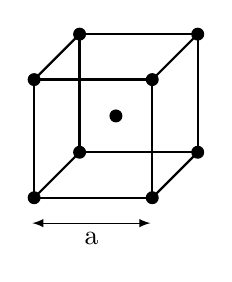
\begin{tikzpicture}[scale=1.5]
  % Disegno del cubo
  \draw[thick] (0,0,0) -- (1,0,0) -- (1,1,0) -- (0,1,0) -- cycle;
  \draw[thick] (0,0,0) -- (0,0,1);
  \draw[thick] (1,0,0) -- (1,0,1);
  \draw[thick] (1,1,0) -- (1,1,1);
  \draw[thick] (0,1,0) -- (0,1,1);
  \draw[thick] (0,0,1) -- (1,0,1) -- (1,1,1) -- (0,1,1) -- cycle;

  % Disposizione delle particelle
  \foreach \x in {0, 1}
    \foreach \y in {0, 1}
      \foreach \z in {0, 1}
        \filldraw (\x,\y,\z) circle (0.05);
   \filldraw (0.5,0.5,0.5) circle (0.05);
   \draw[latex-latex] (-0.4,-0.6)--++(1,0)node[midway, below]{a};
\end{tikzpicture}

        \captionof{figure}{Caption}
        \label{fig:enter-label}
    \end{center}
    dove "a" è la distanza tra due atomi.
\paragraph{Crescita epitassiale}\mbox{}\\
la crescita epitassiale è un processo che consiste nel depositare superficie di un materiale, tipicamente silicio nel caso semiconduttore, un altro strato di materiale differente.
La figura seguente mostra la crescita epitassiale nel caso monodimensionale:
\begin{center}
    \includegraphics{Immagini/imm02.11.2023/HEMT.png}
    \captionof{figure}{Caption}
    \label{fig:enter-label}
\end{center}
La crescita epitassiale si divice in autoepitassia ed eteropitassia. \\
L'autopitassia consiste nella crescita di un substrato perfettamente compatibile a quello di partenza, sia chimicamente che fisicamente.\\
L'eteropitassia, consiste nella crescita di un substato con struttura cristallina poco diversa da quella di partenza.
I materiali che vengono uniti tramite eteropitassia ,devono essere compatibili da diversi punti di vista ( devono essere chimicamente inerti, cioè i due materiali non devono reagire tra loro, poi devono avere coefficiente di espansione termica simile per prevenire la rottura durante raffreddamento e riscaldamento nel processo), ma il nostro interesse si sofferma sul fatto che devono avere un costanti reticolari compatibili.
\end{ripasso}
%
L'eterogiunzione è realizzata facendo crescere uno strato di materiale diverso sopra quello di partenza ponendo attenzione ad aver scelto una combinazione compatibile  perchè cristalli con costanti reticolari troppo diversi possono creare difetti chiamati dislocazioni di adattamento, che agiscono come trappole per elettroni o lacune, rendendo la struttura inadatta per i dispositivi elettronici.
Tuttavia, se la differenza di reticolo tra il substrato e lo strato epitassiale è bassa o zero, è possibile far crescere un cristallo quasi ideale, formando un'eterostruttura. Questa struttura è composta da due materiali diversi con proprietà elettroniche differenti. La discontinuità nel materiale porta a importanti proprietà elettroniche e ottiche, come il confinamento di portatori di carica e il confinamento della radiazione.\\

Le eterostrutture possono avere reticoli accordati (stessa costante reticolare) o avere una leggera discrepanza (fino a circa l'$1\%$), causando una deformazione a trazione o compressione. Si usa il termine eterostrutture pseudomorfe o tese quando c'è una piccola quantità di deformazione, il che può essere vantaggioso per lo sviluppo di dispositivi elettronici ed optoelettronici.

Inoltre, una doppia eterojunzione con uno strato sottile di semiconduttore inserito tra due strati può creare un pozzo di potenziale nella banda di conduzione e/o di valenza, noto come pozzo quantico (QW). Una successione di pozzi quantici debolmente interagenti è chiamata pozzo quantico multiplo (MQW). Se il MQW ha molti strati con un significativo sovrapposizione tra le funzioni d'onda dei pozzi adiacenti, si ottiene un super reticolo (SL), introducendo una periodicità artificiale e modificando le proprietà elettroniche.

\subsection{Leghe di semiconduttori}
Le eterostrutture sono principalmente basate su leghe di semiconduttori.\\
L'idea alla base delle leghe è quella di creare semiconduttori con proprietà intermedie rispetto a quelli già esistenti. Tra queste proprietà vi sono la costante reticolare $a$ e la banda proibita $E_g$. \\
In diversi sistemi materiali, sia $a$ che $E_g$ seguono approssimativamente una legge lineare rispetto ai parametri dei singoli componenti. La motivazione per regolare la costante reticolare è naturalmente quella di ottenere una corrispondenza del reticolo al substrato; \\
la regolazione della banda proibita offre la possibilità di cambiare l'energia dei fotoni emessi, generando lunghezze d'onda importanti, come le lunghezze d'onda di 1.3 o 1.55 µm necessarie per le comunicazioni a fibre ottiche a lunga distanza.\\
Esempi includono leghe composte da due componenti e tre elementi (chiamate leghe ternarie, ad esempio AlGaAs, lega di GaAs e AlAs) e leghe composte da quattro componenti e elementi (chiamate leghe quaternarie, ad esempio InGaAsP, lega di InAs, InP, GaAs, GaP). Selezionando adeguatamente la composizione della lega, è possibile generare leghe semiconduttore che emettono la lunghezza d'onda desiderata e si adattano al substrato giusto.

\[
(M_1N)_x (M_2N)_{1-x} = M_1^x M_2^x N, \quad \text{ad esempio } Al_xGa_{1-x}As
\]
\[
(MN_1)_y (MN_2)_{1-y} = MN_1^y N_2^{(1-y)}, \quad \text{ad esempio } GaAs_yP_{1-y}
\]
dove $x$ e $1-x$ indicano la frazione molare dei due componenti metallici, mentre $y$ e $1-y$ indicano la frazione molare dei componenti non metallici.

La maggior parte delle proprietà delle leghe può essere derivata dalle proprietà dei componenti attraverso un'interpolazione lineare (legge di Vegard) o con correzioni di secondo ordine (legge di Abeles); \\
esempi includono la costante reticolare, la banda proibita, l'inverso delle masse effettive e, in generale, la struttura a bande e le grandezze ad essa correlate.\\
Variando la composizione di una lega ternaria (un grado di libertà) cambia la banda proibita e la lunghezza d'onda correlata, ma, allo stesso tempo, la costante reticolare; in alcuni casi (AlGaAs) i due componenti (AlAs e GaAs) sono già adattati, in modo che le leghe con qualsiasi contenuto di Al siano adatte al substrato (GaAs).

Le leggi di Vegard o Abeles devono essere applicate con attenzione in alcuni casi. Come esempio, consideriamo la lega $Al_x$$Ga_{1-x}As$ e chiamiamo $P$ un parametro della lega, come la banda proibita. La legge di Vegard può essere scritta come:

\[
P(x) = (1 - x)P_{\text{GaAs}} + x P_{\text{AlAs}} \tag{5.1}
\]

\subsection*{Leghe di semiconduttori composti importanti}

Le leghe sono spesso rappresentate come un segmento retto o curvo (per leghe ternarie) o un'area quadrilatera (per leghe quaternarie) in un piano dove la coordinata dell'asse $x$ è la costante reticolare e la coordinata dell'asse $y$ è la banda proibita; \begin{figure}[hbt!]
    \centering
    \includegraphics{Immagini/imm02.11.2023/leghe.png}
    \caption{Caption}%
    \label{fig:enter-label}
\end{figure} 
Gli estremi del segmento e i vertici del quadrilatero sono i componenti semiconduttori; alcune leghe importanti sono riportate di seguito:

\begin{enumerate}
    \item AlGaAs, adatta al reticolo per qualsiasi composizione a GaAs, banda proibita diretta fino a un contenuto molare di Al del 0.45;
    \item InGaAsP, che può essere adattata sia a GaAs che a substrati InP; l'adattamento al substrato InP include la possibilità di emettere lunghezze d'onda di 1.55 o 1.3 µm; la lega è a banda proibita diretta, tranne intorno all'angolo GaP, la cui banda è indiretta;
    \item InAlAs, che può essere adattata al reticolo di InP con una composizione di Al0.48In0.52As;
    \item InGaAs, una lega ternaria adattata a InP con composizione Ga0.47In0.53As; è un sottoinsieme della lega quaternaria InGaAsP;
    \item InGaAsSb, la famiglia degli antimonuri, un possibile materiale per dispositivi a lunghezze d'onda lunghe, ma con una tecnologia piuttosto sottosviluppata rispetto a InGaAsP;
    \item HgCdTe, una lega ternaria particolarmente rilevante per la rivelazione nell'infrarosso lontano (FIR) grazie alla banda proibita molto piccola ottenibile;
    \item SiGe, una lega a banda proibita indiretta importante per le applicazioni elettroniche (transistori bipolari a eterogiunzione) ma anche (in certa misura) per rivelatori e modulatori di elettroassorbimento.
\end{enumerate}

\cleardoublepage
\section{HBT - transistor bipolare a eterogiunzione}
I normli BJT sono costruiti usando un solo tipo di semiconduttore, tipicamente silicio, drogato opportunamente e costruiti con particolari specifiche fisiche per ottenere le caratteristiche tecniche necessarie. Tuttavia il loro guadagno $\beta$ è limitato.
\begin{equation}
    \beta = \dfrac{n_{iE}^2}{n_{iB}^2} \dfrac{N_{DE}}{N_{AB}} \dfrac{W_E}{W_B} \dfrac{D_{nB}}{D_{hE}}
\end{equation}
La precedente equazione verrà riproposta e spiegata successivamente, ora serve solo per fare chiarezza.
Una successiva evoluzione dei normali BJT consiste in transistor costruiti in polisilicio, capaci di sopprimere la corrente di base e quindi ottenere un aumento di guadagno ma anche questi hanno un limite descritto nell'equazione di $\beta$; a parità di concentrazione dei portatori nei semiconduttori intrinseci ($n_i$), gli altri parametri potranno essere modificati per aumentare il guadagno ma alla fine c'è un limite a tutto. La lunghezza $W_B$, per esempio, non può essere resa troppo sottile per evitare il breakdown per perforazione diretta oppure la concentrazione di atomi accettori in base non può essere troppo bassa altrimenti si riduce la conducibilità dei portatori.\\
Alla fine siamo passati alle eterogiunzioni, chiamati HBT (heterojunction bipolar transistor).
I transistor HBT che vedrò saranno di due tipi:
%
\begin{enumerate}
    \item single HBT:
     la giunzione di emettitore e quella base hanno energy gap diversi ($Eg_E \neq Eg_B$), mentre Base e Collettore sono pressoché identiche ($Eg_B \approx Eg_C$).
    \item double HBT:
    la giunzione di emettitore, base e collettore hanno energy gap diversi tra loro ($Eg_E \neq Eg_B\neq Eg_C$).
\end{enumerate}
%
Il principale obiettivo che si pone l'HBT è migliorare le prestazioni ad alta velocità di un transistor bipolare, ottenibile attraverso due strade:
%
\begin{itemize}
    \item sopprimendo l'iniezione di lacune dalla base nell'emettitore per aumentare il guadagno di corrente in continua, $\beta$; 
    \item accelerando il trasporto attraverso la base riducendo il tempo di transito della base, $\tau_B$.
\end{itemize}
%
Il concetto fondmanetale dell'HBT si basa sull'aumento del guadagno di corrente ottenuto utilizzando un semiconduttore per l'emettitore diverso da quello utilizzato per implementare la base, ottenendo così un'eterogiunzione emettitore-base, detto anche Single HBT.\\
%
\cleardoublepage
\subsection{Single HBT}
Base e collettore sono costituiti dallo stesso semiconduttore mentre l'emettitore è fatto di un altro tipo.
\begin{figure}[hbt!]
    \centering
    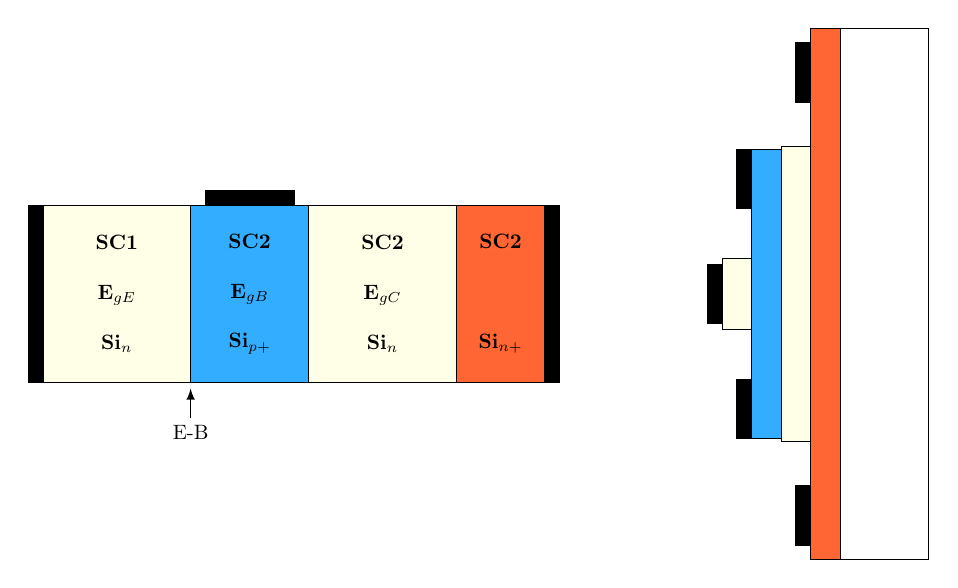
\begin{tikzpicture}[scale=0.75, transform shape]
        \draw[fill=yellow!10!white](0,0) rectangle++(2.5,3) node[pos=0.5,align=center]{$\textbf{SC1}$\\\\$\textbf{E}_{gE}$\\\\$\textbf{Si}_{n}$};
        \draw[fill=blue!40!cyan!80!white](2.5,3)rectangle++(2,-3)node[pos=0.5,align=center]{$\textbf{SC2}$\\\\$\textbf{E}_{gB}$\\\\$\textbf{Si}_{p+}$};
        \draw[fill=yellow!10!white](4.5,0)rectangle++(2.5,3)node[pos=0.5,align=center]{$\textbf{SC2}$\\\\$\textbf{E}_{gC}$\\\\$\textbf{Si}_{n}$};
        \draw[fill=red!50!orange!80!white](7,0)rectangle++(1.5,3)node[pos=0.5,align=center]{$\textbf{SC2}$\\\\\\\\$\textbf{Si}_{n+}$};

        \draw[fill=black](2.75,3) rectangle++(1.5,0.25);
        \draw[fill=black](0,0) rectangle++(-0.25,3);
        \draw[fill=black](8.5,0) rectangle++(0.25,3);

        \draw[latex-] (2.5,-0.1)--++(0,-0.5) node[anchor=north]{E-B};

        \begin{scope}[shift={(15,-3)}, rotate=90]
            \draw(0,0) rectangle++(9,1.5);
            \draw[fill=red!50!orange!80!white](0,1.5) rectangle++(9,0.5);
            \draw[fill=black](0.25,2) rectangle++(1,0.25);
            \draw[fill=black](8.75,2) rectangle++(-1,0.25);

            \draw[fill=yellow!10!white](2,2) rectangle++(5,0.5);
            \draw[fill=blue!40!cyan!80!white](2.05,2.5) rectangle++(4.9,0.5);

            \draw[fill=black](2.05,3) rectangle++(1,0.25);
            \draw[fill=black](6.95,3) rectangle++(-1,0.25);

            \draw[fill=yellow!10!white](3.9,3) rectangle++(1.2,0.5);
            \draw[fill=black](4,3.5) rectangle++(1,0.25);
        \end{scope}
    \end{tikzpicture}
    \caption{Caption}%
    \label{fig:enter-label}
\end{figure}



Considero l'espressione del guadagno di corrente:
\begin{align}
    \beta = \dfrac{I_C}{I_B} \approx \dfrac{I_E}{I_B} = \dfrac{I_{nEB}}{I_{hBE}}
\end{align}
\begin{ripasso}
La corrente che si muove dall'emettitore verso la base è costituita da elettroni. Gli elettroni in base sono portatori minoritari quindi, per quanto visto precedentemente, la corrente di elettroni in base sarà di tipo diffusiva:
\begin{equation*}
    J_{nEB}=qA_nD_{nB} \Delta J_{nEB}
\end{equation*}
Il valore di $J_{nEB}$ si trova partendo dalla legge di azione di massa $n_0 \cdot p = n_{iB}^2$. Dove $n_{iB}$ è la concentrazione degli elettroni nella base in caso di semiconduttore intrinseco.\\
Sapendo che la base è un semiconduttore drogato p, posso approssimare il numero di lacune uguale al numero di atomi accettori impiantati in esso ($p = N_{AB})$, pertanto la concentrazione di elettroni nella base sarà:
\begin{equation*}
    n_0 = \dfrac{n_{iB}^2}{N_{AB}}
\end{equation*}
Ora devo considerare la distribuzione spaziale della concentrazione dei portatori di carica, ottenendo una EDO la cui soluzione è del tipo:
\begin{equation*}
    n(x)=n(0)e^{-x/L_{nB}} 
\end{equation*}
Dove ho inteso $n(0)=n(x=0)=n_0$ la concentrazione di portatori minoritari all'inizio della base.\\
Il ragionamento è analogo per la corrente di lacune dalla base verso l'emettitore.

\end{ripasso}
utilizzando i risultati dell'analisi del BJT, posso scrivere i componenti di corrente in gioco tra base-emettitore. 
\begin{equation}
    I_{nEB}=qA_ED_{nB}\dfrac{d}{dx}\left( \dfrac{n_{iB}^2}{N_{AB}}e^{-x/L_{nB}}\right)e^{V_{BE}/V_T} \approx \dfrac{D_{nB}n_{iB}^2}{W_B N_{AB}}e^{V_{BE}/V_T}
\end{equation}
\begin{equation}
    I_{nBE}=qA_ED_{hE}\dfrac{d}{dx}\left( \dfrac{n_{iE}^2}{N_{DE}}e^{-x/L_{hE}}\right)e^{V_{BE}/V_T} \approx \dfrac{D_{hE}n_{iE}^2}{W_E N_{DE}}e^{V_{BE}/V_T}
\end{equation}
dove si suppone che la lunghezza dell'emettitore, $W_E$, sia breve rispetto a $LpE$. In questo caso, il guadagno di corrente diventa:
\begin{equation}
    \beta = \dfrac{n_{iE}^2}{n_{iB}^2} \dfrac{N_{DE}}{N_{AB}} \dfrac{W_E}{W_B} \dfrac{D_{nB}}{D_{hE}}
\end{equation}
Da questa equazione possiamo capire la vera differenza degli HBT rispetto a un normale BJT, ovvero le concentrazioni di carica:
È importante notare che in un normale BJT accade che i semiconduttori intrinseci su cui si crea la base e l'emettitore siano identici, allora $n_{iB}^2 = n_{iE}^2$. \\
In generale, questa condizione non è vera e il termine $\dfrac{n_{iB}}{n_{iE}}$ non si annulla. \\

Le concentrazioni nel caso più generale sono date da:
\begin{align}
    n_{iB} &= (N_{CB}N_{VB})^{1/2} \cdot e^{-\dfrac{E_{GB}}{2k_BT}} \\
    n_{iE} &= (N_{CE}N_{VE})^{1/2} \cdot e^{-\dfrac{E_{GE}}{2k_BT}}
\end{align}
dove $N_{Cx}$ e $N_{Vx}$ sono rispettivamente la densità equivalente degli stati nei livelli di conduzione e di valenza, valutati per Emettitore e Base.
Inoltre $E_{GB}$ ed $E_{GE}$ fanno riferimento all'energy gap all'interno della base e dell'emettitore.\\
Quindi:

\begin{equation} %non funziona
   \beta = \underbrace{\frac{N_{DE}\ W_E\ D_{nB}}{N_{AB} W_B D_{hE}}}_{\LARGE{\beta^{OMO}}} \left( \dfrac{N_{CB}N_{VB}}{N_{CE}N_{VE}} \right) \cdot e^{\dfrac{E_{GE}-E_{GB}}{k_BT}}
\end{equation}
Da annotare che il termine $\left( \dfrac{N_{CB}N_{VB}}{N_{CE}N_{VE}} \right) \approx 1$ non aiuta con il guadagno di corrente. \\
Ponendo $\Delta E_G =E_{GE}-E_{GB}$ avrò
\begin{equation}
    \beta = \beta^{OMO} e^{\dfrac{\Delta E_G}{k_BT}}= \beta^{HBT}
\end{equation}
posso capire che, implementando l'emettitore con un semiconduttore con un energy gap $E_{GE}$ maggiore (anche di poco) rispetto a $E_{E_G}$ , il $\beta$ aumenta significativamente, poichè il termine è all'esponenziale.\\

Sulla base dell'equazione di $\beta$, l'HBT può essere implementato efficacemente utilizzando diverse strutture di semiconduttori. Tutte fanno riferimento alla relazione esistente tra l'energy gap e la dimensione del reticolo della struttura cristallina riportata in Figura:

\begin{figure}[hbt!]
    \centering
    \includegraphics{Immagini/imm02.11.2023/bandgap of variuos structures.png}
    \caption{Caption}%
    \label{fig:enter-label}
\end{figure}

\begin{figure}[hbt!]
    \centering
    \includegraphics{Immagini/imm02.11.2023/HBT fabbrication.png}
    \caption{Caption}%
    \label{fig:enter-label}
\end{figure}

Il diagramma della banda di energia, riprodotto nella figura successiva per l'AlGaAs/GaAs con singola eterogiunzione, illustra che l'iniezione di elettroni dall'emettitore alla base è favorita rispetto a quella di lacune dalla base all'emettitore a causa della barriera di potenziale significativamente più bassa.



È importante ricordare che tra SC1 ed SC2 cambia la massa ($m*$), da non confondere con la massa efficace.

\cleardoublepage
\subsubsection{Struttura HBT:modello a bande}
\begin{figure}[hbt!]
    \centering
    \includegraphics{Immagini/imm02.11.2023/diagramma a bande HBT.png}
    \caption{Caption}%
    \label{fig:enter-label}
\end{figure}

Il primo transistor eterogiunzione bipolare sperimentale è stato fabbricato nel sistema AlGaAs/GaAs. Questi HBT III-V sono stati sviluppati per applicazioni analogiche ad alta velocità e microonde utilizzando materiali con mobilità degli elettroni molto più elevata rispetto a silicio e germanio. Le combinazioni di materiali III-V più comuni sono riassunte nella Tabella precedente. Il focus principale sulla progettazione dell'HBT III-V era:
\begin{itemize}
    \item sfruttare una grande differenza nell'energy gap tra l'Emettitore e la Base,
    \item ridurre la resistenza della base dopando la base a livelli molto più alti rispetto all'emettitore,
    \item scegliere un materiale con un campo di rottura elevato e una velocità di saturazione elevata nel collettore,
    \item selezionare materiali con banda proibita bassa e alta mobilità degli elettroni per la base.
\end{itemize}

Se $\Delta E_V \uparrow$ di un fattore $\Delta E_C$, allora questo diventa un grande elemento di guadagno perché $I_{PBE} \downarrow$, cioè la corrente dalla base all'emettitore diminuisce e quindi $\beta$ aumenta.

...

Posso avere minori perdite ohmiche in base...

Quali sono i materiali?

È importante sapere che se i semiconduttori diversi avessero "a" diverse, allora farebbero fatica ad agganciarsi. In generale, uno dei due si deve adattare all'altro.

\begin{comment}
    \begin{figure}[h]
    \centering
    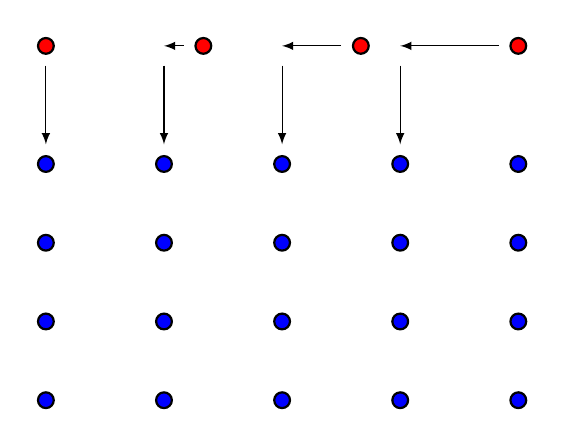
\begin{tikzpicture}[bullet/.style={circle,fill=#1,inner sep=1.5pt}] 
     %\draw (0,0) grid (7,5) \foreach \X in {2,3,4} {\foreach \Y in {1,2,3}
     \def\variable{5}
     % doppio for per creare griglia di blu, ed un rosso fuori dal for Y
     \foreach \X in {1,...,5} {
     
     \foreach \Y in {1,...,4} {
        \node at (1.5*\X,\Y) { \tikz\draw [thick,fill=blue] circle (0.10cm);} 
        ;}
    %if per togliere X=5 del pallino rosso
    \ifnum \X<\variable
     \node at (2*\X-0.5,5.5) { \tikz\draw [thick,fill=red] circle (0.10cm);} 
    \fi
    ;};

      %creo freccie
      \draw[-latex](1.5,5.25)--++(0,-1);

      \draw[-latex](3,5.25)--++(0,-1);
        \draw[-latex](3.25,5.5)--++(-0.25,0);
        
      \draw[-latex](4.5,5.25)--++(0,-1);
         \draw[-latex](5.25,5.5)--++(-0.75,0);

      \draw[-latex](6,5.25)--++(0,-1);
         \draw[-latex](7.25,5.5)--++(-1.25,0);
    \end{tikzpicture}
    \caption{Caption}%
    \label{fig:enter-label}
\end{figure}
\end{comment}

\cleardoublepage
\subsection{HBT - ABRUPT}
Gli HBT abrupt si costruiscono tramite crescita epitassiale in modo da produrre una transizione dal semiconduttore 1 al semiconduttore 2 in modo brusco (da qui il nome abrupt), comportando la formazione di discontinuità nel punto di giunzione.\\
Come regola generale, la banda di conduzione sul lato con gap più ampio giace energeticamente al di sopra di quella sul lato con gap più piccolo, ottenendo la figura sotto riportata.

%
\begin{figure}[hbt!]
    \centering
    \includegraphics{Immagini/imm02.11.2023/eterogiunzione AlGaAs_GaAs.png}
    \caption{Caption}%
    \label{fig:enter-label}
\end{figure}
%
Il diagramma delle bande di energia riprodotto in Figura mostra un HBT AlGaAs/GaAs (o InP/InGaAs) con singola eterogiunzione e mostra come l'iniezione di elettroni dall'emettitore alla base è favorita rispetto a quella di lacune dalla base all'emettitore a causa della barriera di potenziale significativamente più bassa $(\Delta \phi_n < \Delta \phi_n)$ che devono superare.
Quindi gli elettroni non hanno grosse difficoltà nel passare da emettitore a collettore. Al contrario, le lacune risentono della presenza dello "scalino", infatti le lacune vedono un aumento della barriera di potenziale che li separa nel passaggio tra base ed emettitore, comportando la riduzione di queste ultime che effettuano questo salto verso l'emettitore.
A parità di corrente di collettore ,diminuire il transito di lacune da base verso l'emettitore, aumentare il guadagno ad emettitore comune. Questo è il fantaggio di questa soluzione \\
%
\begin{equation}
    \beta \uparrow = \dfrac{I_C}{I_B \downarrow}
\end{equation}
%
L'idea è sfruttare questo ragionamento. Se riuscissimo a massimizzare il $\Delta E_V$ di emettitore rispetto al $\Delta E_g$ si aumenterebbe ancora di più il guadagno perchè, appunto, avrei ulteriormente riddotto il numero di lacune che passano dalla base allemettitore (la probabilità che questi passino).\\

Nei normali BJT Se faccio la base più drogata oppure aumento $W_B$ posso avere il vantaggio di una in resistività più bassa, ma questo implica ridurre il guadagno.
Nel caso HBT invece me ne frego perchè nelle eterogiunzioni, l'effetto della riduzione di beta viene ampiamente compensata dal termine all'espoennziale.

\subsubsection{OSSERVAZIONI}
Di seguito osservazioni che probabilmente non verranno comprese a pieno fino a quando non si avrà strudiato la sezioen HEMT (mosfet con eterogiunzioni).\\

Poiché il rapporto di doping emettitore/base in un HBT tende ad essere basso, la maggior parte della caduta di potenziale elettrostatica si verificherà sul lato meno pesantemente drogato dell'emettitore, e lo spike di potenziale si proietterà sopra la banda di conduzione nella porzione neutra della base, portando a una barriera di potenziale di altezza netta $\Delta EB$. 

Tale barriera ha sia vantaggi che svantaggi.
Consideriamo prima la scalinata di potenziale sul lato della base. 
La tacca può essere interpretata come la creazione di un mini buca di potenziale nel punto di giunzione pertanto,L'ungo la banda di conduzione, la tacca raccoglierà gli elettroni iniettati con il vantaggio di  diminuire le perdite per ricombinazione.

(siccome l'emettitore è drogato meno della base, questa tacca sarà superficiale (5meV))

ma a causa del pericolo di difetti di ricombinazione dell'interfaccia, sarebbe auspicabile eliminare del tutto la tacca applicando all'interfaccia uno strato molto sottile con una concentrazione di accettori molto elevata ($10^{11}/cm^2$). 

Per quanto riguarda la barriera stessa, un piccolo inconveniente della sua esistenza è l'aumento conseguente dell'ordine di $\Delta E_{B}/q$, nella tensione dell'emettitore richiesta per ottenere una data densità di corrente. \\
Abbiamo ora
\begin{equation}
    q(\Delta \phi_p -\Delta \phi_n)=\Delta E_G - \Delta E_B \approx \Delta E_V
\end{equation}
L'ultima uguaglianza si ottiene se la profondità della tacca è piccola rispetto a kT, caso in cui $\Delta EB = \Delta EC$ . Otteniamo quindi
\begin{equation}
    \beta_{max}=\dfrac{N_{DE}}{N_{AB}}\dfrac{v_{nh}}{v_{hn}}\exp(\Delta E_V/k_BT)
\end{equation}
Se la discontinuità della banda di valenza è sufficientemente grande, rimane un miglioramento significativo. Sfortunatamente, nel sistema di maggior interesse attuale, il sistema (Al,Ga)As/GaAs, la discontinuità della banda di valenza è piuttosto piccola, $\Delta EV = 0.15 \Delta Eg$, e la riduzione dello spike da gradiente è probabilmente essenziale.
Gli svantaggi sopra menzionati della barriera di potenziale aggiuntiva che accompagna una giunzione emettitore/base abrupt sono parzialmente compensati dal fatto che tale barriera inietterà gli elettroni nella regione della base con una notevole energia cinetica e quindi con una velocità molto elevata ($10^8$ cm/s). A causa della dipendenza direzionale della scattering da fonone ottico polare che è il processo di scattering dominante nei composti III/V, sono richieste diverse collisioni prima che gli elettroni perdano la loro elevata velocità in avanti. Il risultato dovrebbe essere un trasporto di elettroni quasi balistico altamente efficiente e molto veloce attraverso la base. Esattamente quale sarà l'equilibrio tra svantaggi e benefici per la giunzione emettitore/base abrupt rispetto a quella gradita, rimane da vedere. Ma sembra probabile che gli effetti balistici troveranno la loro strada nei futuri transistori progettati specificamente attorno a essi.\\
```%
\\
In questo diagramma a bande è complicato riuscire a calcolare le correnti che passano da una parte o dall'altra.\\
Quello che tipicamente viene accettato è che la densità di corrente di elettroni emessi da emettitore verso la base sia moltiplicata per una velocità detta velocità di transito in base, inoltre èmoltiplicato per una quantità esponenziale che tiene conto di quanto è costante in banda.\\
più la banda è larga, meno elettroni ci staranno dall'altra parte($e^{-\Delta E_C}$) $->$ è un termine la cui presenza non si dimostra ma è accettato come un fatto assiomatico (è detto termine di selezione che selezioni i livelli di energie i cui elettroni possono andare dall'altra parte).\\
poi c'è un termine di emissione: $ e^{\dfrac{V_{BE}}{V_T}}$.
.
c'è quindi un termine di emissione (e*-deltaEc) che seleziona le energiae degli elettronic che possono andare dall'altra aprte e poi untermine di emissione.
\begin{equation}
    J_{nEB} = q \dfrac{n_{iB}^2}{N_{AB}} \cdot v_{TB} \cdot e^{-\Delta E_C} \cdot e^{\dfrac{V_{BE}}{V_T}} 
\end{equation}
vtb è la velocità di transito in base.\\

L'equazione delle lacune è relativamente più facile e obbedisce alla formula della corrente di diffusione
\begin{equation}
    J_{pBE} = q \dfrac{n_{iE}^2}{N_{DE}} \dfrac{D_p}{W_E} \cdot e^{\dfrac{V_{BE}}{V_T}}
\end{equation}
risistemo le equazioni e ricordo che $n_i$ dipende dall'energy gap, inoltre ho che:

\begin{equation}
    \Delta E_g = \Delta E_V + \Delta E_C
\end{equation}
si scopre che:
\begin{equation}
    \beta = \dfrac{N_{DE}}{N_{AB}} \dfrac{v_{TB}}{D_P/W_E} e^{\dfrac{\Delta E_g - \Delta E_C}{k_B T}}=\dfrac{N_{DE}}{N_{AB}} \dfrac{v_{TB}}{D_P/W_E} e^{\dfrac{\Delta E_V}{k_B T}}
\end{equation}\\
Quindi alla fine, il vero responsabile dell'innesco dell'effetto etrogiunzione è..
Nei dispositivi HBT abrupt (che sono quelli che hanno prevalentemente un substrato di ossido di gallio GaAs) succede che .. (?)

la frazione molare mi impone certi limiti. per non rompere la giunzione tra alluminio ed gallio, tipicamente si usa x=0.3 ovvero circa il 30% rispetto alla frazione molare di gallio

la velocità di transito lo si aumenta diminuendo significativamente lo spessore della base.
Per questo dispositivi ad alta velocità


\cleardoublepage
\subsection{Graduali}
E' possibile sfruttare le eterogiunzioni per per risolvere problemi differenti rispetto al solo aumento del guadagno di corrente.
In particolare vedrò sotto alcune spiegazioni su come ridurre la tensione di offset (mandare $V_{CE}=0$ quando $I_C=0$? e altro.
Comunque la risposta si ottiene mendiante una doppia eterogiunzione.

\subsubsection{Double HBT}
nei double HBT varrà la condizione $E_g^E > E_g^B$ ed $E_g^C > E_g^B$. \\
i vantaggi di questa soluzione sono principlamente due:
%
\begin{itemize}
    \item Si riduce la $V_{CE}^{sat}$, più comunemente chiamata tensione di offset (Vos),  perchè la $V_{CE}$ applica, a tutti gli effetti, un offset sulla tensione di uscita dal transistor: \\
    
    grafico ideale e offset

    \item Si aumenta la tensione di breakdown, Importante per la gestione di segnali analogici ad alta frequenza.
\end{itemize}

Quando sono nei pressi della saturazione, il diagramma a bande è il seguente:
\begin{figure}[hbt!]
    \centering
    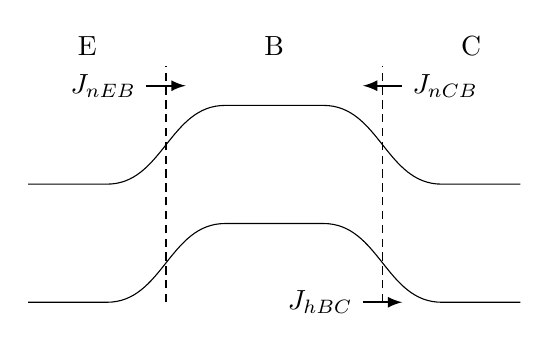
\begin{tikzpicture}[scale=0.5]
        %grafico sopra
        \draw (0,3)--++(2,0) to [in=180, out=0] ++(3,2)
         --++(2.5,0) to [in=180, out=0] ++(3,-2)--++(2,0); 

        %grafico sotto
        \draw (0,0)--++(2,0) to [in=180, out=0] ++(3,2)
         --++(2.5,0) to [in=180, out=0] ++(3,-2)--++(2,0); 

         %altro
         \draw[densely dashed](3.5,0)--++(0,6);
         \draw[densely dashed](9,0)--++(0,6);

         %freccie e label correnti
         \draw [latex-,thick](4,5.5)--++(-1,0)node[left]{$J_{nEB}$};
         \draw [latex-,thick](8.5,5.5)--++(1,0)node[right]{$J_{nCB}$};
         \draw [-latex,thick](8.5,0)node[left]{$J_{hBC}$}--++(1,0);

         \node at (1.5,6.5) []{E};
         \node at (6.25,6.5) []{B};
         \node at (11.25,6.5) []{C};
         
    \end{tikzpicture}
    \caption{Caption}%
    \label{fig:enter-label}
\end{figure}

ho visto e rivisto le formule:
\begin{align}
    J_{nEB} &= \dfrac{n_{iB}^2}{N_{AB}} \dfrac{D_n}{W_B} e^{\dfrac{q(V_B - V_E)}{V_T}}\\
    J_{nCB} &= \dfrac{n_{iB}^2}{N_{AB}} \dfrac{D_n}{W_B} e^{\dfrac{q(V_B - V_C)}{V_T}}\\
    J_{hBC} &= \dfrac{n_{iC}^2}{N_{DC}} \dfrac{D_p}{W_C} e^{\dfrac{q(V_B - V_C)}{V_T}}\\
\end{align}
Affinchè la tensione di offset vada a zero è necessario che si annullino tutte le correnti, ovvero che:
\begin{equation}
    \left. J_C \right |_{V_C=0} = J_{nEB} - J_{nCB}- J_{hCB} = 0
\end{equation}
%
Assumendo che anche l'emettitore sia posto a massa ($V_E=0$), trovo che $J_{nEB}$ e $J_{nCB}$ andranno a zero, purtroppo però $J_{hBC}$ non è piccolo. Questa corrente è il principale contributo alla tensione di offset, cioè è l'unica corrente prente qando $V_C=0$
\begin{ricevimento}
    cos'è che deve essere zero. Ve e Vc o  solo una delle due?
\end{ricevimento}

Uno dei metodi migliori per ridurre $J_{hBC}$ è quello di ridurre la concentrazione degli intrinseci nel collettore ($n_{ic}$ e per fare questo è necessario aumentare il suo energy gap. Questo è intuitivo osservando l'equazione
\begin{equation}
    n_{ic}^2=N_{VC}\ N_{CC}\ e^{-\dfrac{\Delta E_{gC}}{k_BT}}
\end{equation}
Di conseguenza
\begin{align}
    J_{hBC} \downarrow &= \dfrac{n_{iC}^2 \downarrow}{N_{DC}} \dfrac{D_p}{W_C} e^{\dfrac{q(V_B - V_C)}{V_T}}\\
\end{align}
Questo è il motivo per cui si usano eterogiunzioni anche tra base e collettore

%
\subsubsection{Struttura esempio di un HBT}
Questi HBT sono strutture verticali che si costruiscono a partire da un substrato, solitamente un semiconduttore con elevato $E_{gap}$ (cioè più isolante di altri). Un esempio di questi dispositivi è mostrato nella figura seguente:\\

\begin{figure}[hbt!]
    \centering
    \begin{tikzpicture}
    
    %disegno i vari strati colorati blu/rosso
        \draw(0,0) rectangle++(10,2);
        \draw[pattern=north east lines, pattern color= blue](0,2) rectangle++(10,0.25);
        \draw[pattern=north east lines, pattern color= red](0,2.25) rectangle++(10,0.25);
        \draw[pattern=north east lines, pattern color= blue](0,2.5) rectangle++(10,0.25);
        \draw[pattern=north east lines, pattern color= red](0,2.75) rectangle++(10,0.25);
        \draw[pattern=north east lines, pattern color= blue](0,3) rectangle++(10,0.25);
        
        %C2 n+GeAs
        \draw[](0,3.25) rectangle++(10,0.5)node[pos=.5]{n+, GeAs};
        %C1 n, GeAs
        \draw[](2.5,3.75) rectangle++(5,0.5)node[pos=.5]{n, GeAs};
        %metallizzazione sinistra C e label
        \draw[pattern=north east lines , pattern color=black](0,3.75) rectangle++(2,0.25);
        \draw (1,4) to [short,-*]++(0,0.25)node[right]{C};
        %metallizzazione destra C e label
        \draw[pattern=north east lines , pattern color=black](8,3.75) rectangle++(2,0.25);
        \draw (9,4) to [short,-*]++(0,0.25)node[right]{C};
        
        %rect viola= BUFFER
        \draw[pattern=north east lines, pattern color= violet](2.5,4.25) rectangle++(5,0.25)node[pos=.5]{\textbf{BUFFER}};
        %B p GeAs
        \draw[](2.5,4.5) rectangle++(5,0.5)node[pos=.5]{p, GeAs};
        %metallizzazione sinistra B e label
        \draw[pattern=north east lines , pattern color=black](2.5,5) rectangle++(1,0.25);
        \draw (3,5.25) to [short,-*]++(0,0.25)node[right]{B};
        %metallizzazione destra B e label
        \draw[pattern=north east lines , pattern color=black](6.5,5) rectangle++(1,0.25);
        \draw (7,5.25) to [short,-*]++(0,0.25)node[right]{B};
        
        %E
        \draw[](4,5) rectangle++(2,0.5)node[pos=.5]{n+, GeAs};
        \draw[](4,5.5) rectangle++(2,0.2);
        %metallizzazione E e label
        \draw[pattern=north east lines , pattern color=black](4,5.7) rectangle++(2,0.25);
        \draw (5,5.95) to [short,-*]++(0,0.25)node[right]{E};
        
        %disegno freccie e labeldegli strati
        \draw[latex-](10.1,2.125)--++(0.25,0)node[right]{\small{$GeAs$}};
        \draw[latex-](10.1,2.4)--++(0.5,0)node[right]{\small{$AlGeAs$}};
        \draw[latex-](10.1,2.625)--++(1,0)node[right]{\small{$GeAs$}};
        \draw[latex-](10.1,2.875)--++(1.25,0)node[right]{\small{$AlGeAs$}};
        \draw[latex-](10.1,3.125)--++(1.5,0)node[right]{\small{$GeAs$}};
        %altri label
        \node at (0.5,3.5) []{C2};
        \node at (2.95,4) []{C1};
        \node at (2.95,4.75)[]{B};
        %label nascosto per centrare figura
        \draw[latex-,white](-0.1,3.125)--++(-1.5,0)node[left]{\small{$GeAs$}};
        %asse Z
        \draw[-latex](-0.75,0)--++(0,5) node[left]{z};
    \end{tikzpicture}
    \caption{Caption}%
    \label{fig:enter-label}
\end{figure}
In questo HBT è possibile notare diverse cose,. Innanzitutto C2 è un subcollettore GaAs drogato n+ utilizzato per risolvere tutta quella teoria delle giunzioni radrizzanti viste nelle giunzioni metallo-SC.
Sopra C2 viene costruito il vero collettore C1, drogato n-GaAs ed a la funzione di ridurre l'effetto early e la capacità di giunzione.\\
Sopra C1 è stata fatta una crescita epitassiale per creare un buffer
\begin{ricevimento}
    il buffer a che serviva?
\end{ricevimento}
Guardando da C2 verso il substrato, vedo delle strutture di semiconduttori intrinseci di materiale alternato. Sono scelti in modo creare nella banda di energia degli intervalli di energy gap + alto seguiti da energy gap più basso, creando quello che si definisce "super reticolo":
\begin{figure}[hbt!]
    \centering
    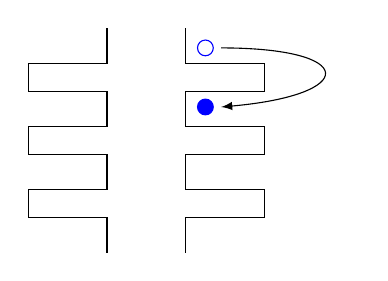
\begin{tikzpicture}
       \draw[](+0.5,0)--++(0,-0.45)--++(+1,0)--++(0,-0.35)--++(-1,0)--++(0,-0.45)--++(+1,0)--++(0,-0.35)--++(-1,0)--++(0,-0.45)--++(+1,0)--++(0,-0.35)--++(-1,0)--++(0,-0.45);
    \begin{scope}[xscale=-1]
        \draw[](+0.5,0)--++(0,-0.45)--++(+1,0)--++(0,-0.35)--++(-1,0)--++(0,-0.45)--++(+1,0)--++(0,-0.35)--++(-1,0)--++(0,-0.45)--++(+1,0)--++(0,-0.35)--++(-1,0)--++(0,-0.45);
    \end{scope}

    %disegno elettrone
    \draw [blue] (0.75,-0.25) circle (0.1);
    \draw [-latex](0.95,-0.25) to [out=0,in=5,distance=1.75cm](0.95,-1);
    \draw [blue, fill=blue] (0.75,-1) circle (0.1);
    \end{tikzpicture}
    \caption{Caption}%
    \label{fig:enter-label}
\end{figure}
\begin{ricevimento}
    fare diagramma a bande. chiedere confronto e chiedere a che serve superreticolo tra C e substrato.
    il superreticolo è usato come alternativa al DTI, per isolare da eventuali dispositivi adiacenti, giusto?
\end{ricevimento}
Il super reticolo è un metodo usato per isolare il collettore (C2) dal substrato permettendo l'integrabilità di un numbero maggiore di dispositivi sopra uno stesso substrato.
In parole povere serve a sostituire il DTI (è spiegato nel HBT SiGE), la trincea di isolante. infatti, il super reticolo  ha la funzione di bloccare gli gli eventuali elettroni che potrebbero fluire dal collettore C2 al substrato. Trovando queste trappole artificiali, gli elettroni rimangono confinate e non fluiscono nel substrato.
E' usato al posto del DTi perchè favorisce una maggiore integrazione
\begin{ricevimento}
    altri motivi per cui sostituire il DTI con super reticolo?
\end{ricevimento}

per fare un riepilogo brevissimo:\\
I BJT sono per costruzione (ma neanche tanto) dei dispositivi veriticali ed hanno carateristiche diverse rispetto ai MOS:
\begin{enumerate}
    \item La densità di corrente dei BJT è più alta
    \item Le cariche nella giunzione sono meno affetti dal rumore che si innesca quando attraversa la giunzione.
    \begin{ricevimento}
        chiarire
    \end{ricevimento}
    \item In generale i BJT sono più complicati dei MOS
\end{enumerate}

\section{6.11.2023}
\subsection{STRUTTURA HBT Si-Ge:}
%
Di seguito si vede la struttura di un transistor bipolare:
\begin{figure}[hbt!]
    \centering
    \includegraphics[width=0.35\textwidth,angle=90]{Immagini/imm06.11.2023/HBTSiGe_06_11_2023.jpg}
    \caption{Caption}%
    \label{fig:enter-label}
\end{figure}
%
Si costruisce su un substrato di tipo p ,tramite crescita epitassiale, alternado le caratteristiche chimiche e di drogaggio del semiconduttore modificando le frazioni molari.\\
Il primo strato che si nota è il sub-collettore di tipo n+, che successivamente viene accresciuto con uno strato più stretto che è il collettore vero e proprio ed è drogato tipo n.\\
Sia sub-collettore che collettore sono un po’ più stretti del substrato p.\\
Sopra c’è la base in Silicio-Germanio e sopra ancora c'è l’emettitore in Silicio. \\
Di fianco c’è un’inserzione verticale, una trincea che si chiama “deep trench isolation” (DTI) che parte dal substrato p e arriva all’emettitore e serve per isolare dispositivi adiacenti. Poi c’è una seconda trincea di isolamento che parte dal sub-collettore e arriva all’emettitore e si chiama “shallow trench isolation”, STI.\\
Sopra la STI poggiano i contatti metallici di base mentre il contatto di collettore è a fianco della deep trench.\\
Poi si costruisce dell’ossido (quello a pallini) e sopra lo strato di emettitore si mette del poly-silicio su cui poi si và a fare la metallizzazione di emettitore.\\
Si usa il il poly-silicio perché è più resistente alle temperature e fa un buon contatto elettrico, quando devi fare un contatto ohmico molto piccolo è preferibile non mettere il metallo direttamente sulla giunzione, ma interporci uno strato di poly-silicio che diventa un’estensione dell’emettitore sulla quale depositare il metallo, ma l’area di emettitore è comunque quella definita dalla giunzione base-emettitore.\\
Anche le DTI sono fatte di ossido, alla destra dell’ossido di destra c’è un contatto metallico sopra un pozzo p+ e un secondo STI, questo è il contatto del substrato.\\
%
Se sono in presenza di un npn si ha la coppia di giunzioni caratteristica dell’elemento attivo e una terza giunzione che va al substrato. In blu la parte attiva del transistor, il resto sono parassiti.\\
%
\begin{wrapfigure}{r}{0.5\textwidth} % L'opzione {l} posiziona l'immagine a sinistra, 0.5\textwidth indica la larghezza
  \centering
  \includegraphics[width=0.35\textwidth,angle=90]{Immagini/imm06.11.2023/CircEq_06_11_2023.jpg}
  \caption{Didascalia dell'immagine}
\end{wrapfigure}
%
Spesso viene messo a disposizione il contatto di substrato perché è importante che le giunzioni che si vengono a creare siano interdette infatti, può capitare che ci siano delle correnti nel stubstrato che possono attivare il dispositivo.
Potrei pensare di collegare il substrato direttamente a massa ma il problema è che non è garantito che con la semplice connessione a ground, localmente tutti i dispositivi abbiano polarizzazione tale da garantire che quella terza giunzione sia interdetta. 
Quindi fai in modo da porre localmente quella giunzione a ground.
Questo è usato soprattutto nei MOS quando interconnetti fra loro molti dispositivi in topologie complesse.
\begin{ricevimento}
    chiarire
\end{ricevimento}

\cleardoublepage
\subsection{Teoria delle bande del HBT Si-Ge:}
L'HBT silicio-germanio sfutta la teoria del graded HBT.
In queste strutture viene fatta una modulazione del contenuto della frazione molare di germanio sulla base, in funzione della direzione z secondo la formula:
\[HBT - Si_xGe_{1-x}\]
\begin{minipage}{.6\textwidth}
\vspace{0pt}
L'andamento della frazione moltare è mostrato nella figura.\\
In esso osservo come la frazione molare, in funzione della profondità z, ha inizialmente un profilo con andamento crescente e poi, verso la fine della base, decresce. Tratteggiato c’è il profilo del  drogaggio
\end{minipage}
\begin{minipage}{.4\textwidth}
    \begin{center}
        \includegraphics[width=0.45\textwidth,angle=90]{Immagini/imm06.11.2023/FrazMolSiGe_06_11_2023.jpg}
    \captionof{figure}{Didascalia dell'immagine}
    \end{center}
\end{minipage}
%
(è meglio la figura di filippo, non questa)
Per vedere la differenza tra caso con profilo graduale e BJT, faccio il diagramma a bande come se il Germanio non ci fosse e sopra aggiungo il profilo della banda in presenza di germanio.
%
\begin{figure}[hbt]
    \centering
    \includegraphics[width=0.25\textwidth,angle=90]{Immagini/imm06.11.2023/BandeSiGe_06_11_2023.jpg}
    \caption{Caption}%
    \label{fig:enter-label}
\end{figure}\\
%
La presenza del germanio graduale fa sì che l’energy gap diminuisca in modo altrettanto graduale.
L'energy gap diminuisce perchè il Silicio ha Eg=1.14 e il Germanio ha energy gap minore Eg=0.707, quindi è normale che verso la fine della base (in prossimità del collettore), laddove la concentrazione di germanio è maggiore di quella del silicio.

Ora osservo le varie implicazioni di questa struttura.
Le lacune nn subiscono alcuna modifica, ma gli elettroni beneficiano di un campo elettrico addizionale che li spingono verso il collettore. Si crea in base un campo elettrico che prima non c’era.

 Questa è la chiave di volta degli HBT: modulare il Germanio in base significa modulare il diagramma a bande e instaurare un campo elettrico che facilita il moto degli elettroni. 
 Facilitare il moto degli elettroni si porta dietro molte caratteristiche migliorative.

 L’incremento di Eg nella base della eterogiunzione ha un andamento lineare che dipende da 
\[\Delta Eg_{max}\]
\begin{align}
    \Delta Eg_{(Si-Ge,BASE)}(z)=\dfrac{z}{W_B}\Delta Eg_{max} \\
    \Delta Eg_{max} \approx100meV
\end{align}
La descrizione della corrente degli intrinseci non è più semplice. Dipende da come viene fatto crescere il Germanio nella base.
\begin{equation}
    J_C=\dfrac{qe^{V_{BE}/V_T}}{\bigintss_{0}^{W_B}\dfrac{Pp(x)}{D_{niB} \cdot n_{iB}^2(x)}dx}
\end{equation}
%
dove:
%
\begin{equation}
    n_{i}^2(SiGe,z)=n_i^2(Si)e^{\dfrac{\Delta E_{giBsiGe(z)}}{k_BT}}
\end{equation}
%
\begin{exbox}[come ho ottenuto la formula della corrente precedente?]
    spiegazione da mettere
\end{exbox}
%
La corrente di collettore è una funzione della posizione, dipende da z, come anche la corrente di base:
%
\begin{equation}
    J_B=\dfrac{qe^{V_{BE}/V_T}}{\bigintss_{0}^{W_B}\dfrac{N_{DE}(x)}{D_{p}\cdot n_{iE}(x)^2}dx}
\end{equation}
%
Da queste posso trarre delel prime conclusioni che mi permettono di distinguere i benefici del HBT SiGe da un normale BJT in SI:
\begin{enumerate}
    \item il guadagno di corrente è maggiore: $\beta_{(SiGe)}\approx 4 \beta_{(Si)}$
    Si ottiene considerando:
    \begin{equation}
    \beta_{(SiGe)}=\dfrac{J_C}{J_B}\approx \dfrac{\Delta E_{gmax}}{k_BT}=4 
    \end{equation}
    Nell’ipotesi che $\Delta Eg$, max sia dell’ordine dei 100 meV, ti viene che il nuovo $/beta$ è circa quattro volte il $/beta$ del Silicio standard;

    \item La tensione di Early è maggiore: $V_{Early}^{(SiGe)} \approx 10 \cdot V_{Early}^{(Si)}$
    \begin{equation}
    \dfrac{V_{Early}^{(Si_Ge)}}{V_{Early}^{(Si)}}\approx \dfrac{e^{\dfrac{E_{gmax}}{k_BT}}}{\dfrac {E_{gmax}}{k_BT}} 
    \end{equation}

    \item Il tempo di transito in base è minore: $\tau_B^{(SiGe)}= [0.5 \div 0.3] \tau_B^{(Si)}$
    \begin{equation}
    \dfrac{\tau_B^{(SiGe)}}{\tau_B^{(Si)}}\approx \dfrac{k_BT}{\Delta E_{gmax}}\left[ 1-\dfrac{k_BT}{\Delta E_{gmax}} \left( 1-e^{-\dfrac{k_BT}{\Delta E_{gmax}}}\right)\right] \approx \dfrac{1}{2}
    \end{equation}
\end{enumerate}

Quindi utilizzando una struttura verticale è possibile inserire gradualmente frazioni molari del germanio, modificando di conseguenza il diagramma a abnde. L'impatto si ha sulla concetrazione degli intrinseci che a castata impatta principlamente sui parametri come $\beta$, agendo sulla $J_C$, $V_{Early}^(SiGe)$ detta $V_{A}$ e sulla $\tau_B^{(SiGe)}$

Anche gli hbt sono soggetti all'effetto kirk cioè hanno effetti di riduzione del prodotto guadagno banda in funzioen della decrescita di $\beta$ per allargamento di $W_B$

grafico ft-Jc



\cleardoublepage

\section*{27.11.2023}
La struttura realizzativa di partenza è mostrata nella seguente figura, accanto al diagramma a bande:
%
\begin{figure}[hbt!]
    \centering
    \begin{circuitikz}
        \draw (0,0) rectangle ++ (6,2) node[pos=0.5]{$GaAs-i$};
        \draw (0,2) rectangle ++ (6,1) node[pos=0.5]{$Al_{0.3}Ga_{0.7}A_s-n^+$};

        %metalizzazioni
        \draw[pattern = north east lines, pattern color = black] (2,3) rectangle ++(2,0.25);
        \draw(+3,3.25)to[short,-*]++(0,0.2) node[right]{G};
        
        \draw[pattern = north east lines, pattern color = black] (0,1.5) rectangle ++(-0.2,1) ;
        \draw(-0.2,2)to[short,-*]++(-0.2,0) node[left]{S};
        
        \draw[pattern = north east lines, pattern color = black] (6,1.5) rectangle ++(+0.2,1);
        \draw(+6.2,2)to[short,-*]++(+0.2,0) node[right]{D};
        %massa
        \draw[pattern = north east lines, pattern color = black] (0,0) rectangle ++(6,-0.15);
        
        \draw (3,-0.15) to (3,-0.2) node[ground]{};

        %disegno i tratteggi per il diagramma a bande
        \draw[densely dotted] (9,3)--++(6,0);
        \draw[densely dotted] (9,2)--++(6,0);
        \draw[densely dotted] (9,0)--++(6,0);
        \draw[densely dotted] (12,4)--++(0,-4.5)node[anchor=north]{\footnotesize{Ef}};
        \draw[densely dotted] (12.75,0)--++(0,-0.5)node[anchor=north]{\footnotesize{Ec}};
        \draw[densely dotted] (11.25,0)--++(0,-0.5)node[anchor=north]{\footnotesize{Ev}};
        
        % disegno diagramma a bande 
        \draw(13.5,3) to [in=155, out=181,distance=1cm](12.5,2); 
        \draw(10.75,3) to [in=155, out=181,distance=1cm](9.75,2); 
        
        \draw(11.5,2) to [in=90, out=340](12.75,0);
        \draw(10,2) to [in=90, out=340](11.25,0);

        %disegno pozza di elettroni
        \draw[pattern=north east lines, pattern color=blue](11.5,2) to [in=145, out=340](12,1.74)--(12,2)--cycle{};

        %disegno cariche positive
        \node at (12.19,2.10) { \tikz\draw [thick,red, scale=1.25]
        (-0.05,0)--(0.05,0) (0,0.05)--(0,-0.05);};
        \node at (12.08,2.27) { \tikz\draw [thick,red, scale=1.25]
        (-0.05,0)--(0.05,0) (0,0.05)--(0,-0.05);};
        \node at (12.07,2.5) { \tikz\draw [thick,red, scale=1.25]
        (-0.05,0)--(0.05,0) (0,0.05)--(0,-0.05);};
        \node at (12.2,2.7) { \tikz\draw [thick,red, scale=1.25]
        (-0.05,0)--(0.05,0) (0,0.05)--(0,-0.05);};
        \node at (12.4,2.85) { \tikz\draw [thick,red, scale=1.25]
        (-0.05,0)--(0.05,0) (0,0.05)--(0,-0.05);};

        %disegno cariche negative
        \node at (12.3,2.3) { \tikz\draw [thick,blue, scale=1.25]
        (-0.05,0)--(0.05,0);};
        % label
        \draw[|-|](12,3.5)--++(1.5,0) node[anchor=south east]{$qV_{bi}$};
        
        \draw[|-|,color=violet!50!white](11.5,2)--(12.5,2);
        \draw[|-|,color=violet!80!white](9.75,2)--(10,2);
        \draw[->,color=violet!50!white](12.30,1.9) to [in=180, out=300] (13,1.75)node[right]{\footnotesize{discontinuità}};
        %per centrare tutto metto un alinea bianca a sx
        \draw[white](15,0)--++(1,0);
    \end{circuitikz}
    \caption{Struttura di un HEMT}
    \label{fig:Struttura di un HEMT}
\end{figure}
\\%
\noindent\begin{minipage}{0.49\textwidth}
Il diagramma a bande vale nel caso di assenza di polarizzazione ($V_G=0 Volt$).\\
Si noti la differenza rispetto al diagramma a bande per una struttura ad omogiunzione (tutti i SC sono GaAs) nel quale si avrebbe un andamento ,dentro lo strato superiore, che si raccorda in modo perfetto con quello inferiore dello dello strato intrinseco. Nel caso dell'eterogiunzione inceve, la presenza del meteriale AlGaAs provoca una discontinuità nelle bande (di valore $\Delta E_c$) a causa del differente energy gap rispetto a quello del GaAs intrinseco.\\
\end{minipage}
\hfill
\begin{minipage}{0.52\textwidth}\raggedleft
    \begin{tikzpicture}
        % disegno diagramma a bande 
        \draw(13.5,3) to [in=155, out=181,distance=1cm](12.5,2); 
        \draw(10.75,3) to [in=155, out=181,distance=1cm](9.75,2); 
        
        \draw(11.5+1,2) to [in=90, out=340](12.75+1,0);
        \draw(10-0.25,2) to [in=90, out=340](11.25-0.25,0);

        

        %disegno cariche positive
        \node at (12.19,2.10) { \tikz\draw [thick,red, scale=1.25]
        (-0.05,0)--(0.05,0) (0,0.05)--(0,-0.05);};
        \node at (12.08,2.27) { \tikz\draw [thick,red, scale=1.25]
        (-0.05,0)--(0.05,0) (0,0.05)--(0,-0.05);};
        \node at (12.07,2.5) { \tikz\draw [thick,red, scale=1.25]
        (-0.05,0)--(0.05,0) (0,0.05)--(0,-0.05);};
        \node at (12.2,2.7) { \tikz\draw [thick,red, scale=1.25]
        (-0.05,0)--(0.05,0) (0,0.05)--(0,-0.05);};
        \node at (12.4,2.85) { \tikz\draw [thick,red, scale=1.25]
        (-0.05,0)--(0.05,0) (0,0.05)--(0,-0.05);};

        %disegno cariche negative
        \node at (12.3,2.3) { \tikz\draw [thick,blue, scale=1.25]
        (-0.05,0)--(0.05,0);};
        % label
        \draw[|-|](12,3.5)--++(1.5,0) node[anchor=south east]{$qV_{bi}$};
        
        \draw[|-|,color=violet!50!white](11.5,2)--(12.5,2);
        \draw[|-|,color=violet!80!white](9.75,2)--(10,2);
        \draw[->,color=violet!50!white](12.30,1.9) to [in=180, out=300] (13,1.75)node[right]{\footnotesize{NON c'è discontinuità}};
        %per centrare tutto metto un alinea bianca a sx
        \draw[white](15,0)--++(1,0);
    \end{tikzpicture}
    \captionof{figure}{omogiunzione}
\end{minipage}
\begin{ricevimento}
    chiedere aiuto per sistemare le figure. come sarebbe quella omogiunzione? quello dell'eeterogiunzion ega Vg=0 oppure no?
\end{ricevimento}
La tensione $V_{bi}$ dipende dalla differenza nel lavoro di estrazione che c'è tra metallo e semiconduttore.
L'andamento che assumono i livelli di conduzione e valenza sono spiegati tramite le teorie studiate:
\begin{itemize}
    \item l'andamento nella giunzione Metallo-SC è quello di una giunzione schottky: gli elettroni del SC $AlGaAs_n^+$ saltano verso il metallo lasciandosi dietro ioni fissi positivi e creando quindi una regione di svuotamento nel SC, pertanto il livello di fermi del SC scende fino ad allinearsi a quello del metallo creando una curvatura della banda SC $AlGaAs_n$ rivolta verso l'alto.
    \item un'altro accumulo di ioni fissi positivi si verifica nella giunzione $AlGaAs_n^+$-$GaAs_i$: gli elettroni del SC $AlGaAs_n^+$ saltano verso il SC $GaAs_i$ perchè ha livello di fermi minore. Essendo però un'eterogiunzione, il loro diverso energy gap comporta la formazione di una buca di potenziale durante il livellamento dell'energia di fermi. Quindi gli elettroni saltano dall'interfaccia di $AlGaAs_n$ verso la buca di potenziale situata in $GaAs_i$, lasciando dietro ioni fissi positivi e quindi una regione di svuotamento.
\end{itemize}

Il layer superiore è denominato "supply layer" poiché genera un sottile canale nel substrato attraverso il quale gli elettroni mobili possono muoversi. La densidtà di carica che si trova all'interno del canale è chiamato "$n_s$.
Da notare come il riempimento del canale non è dovuto da meccanismi elettrostatici come nel caso MOSFET ma da motivi fisici legati al livello di fermi che portano alla formazione di un canale a sezione triangolare.\\
In questa specifica configurazione, il semiconduttore in cui avviene tale movimento è intrinseco, garantendo una mobilità elevata degli elettroni.\\ 
Effettuando uno zoom sulla banda di conduzione dell'eterogiunzione, è possibile notare che gli elettroni in arrivo nella buca di potenziale occupano livelli energetici discreti (ad esempio: $E_1,E_2,E_3$). \\


\newpage
Faccio uno zoom non in scala e lo proietto orizzontalmente:

    \begin{center}
    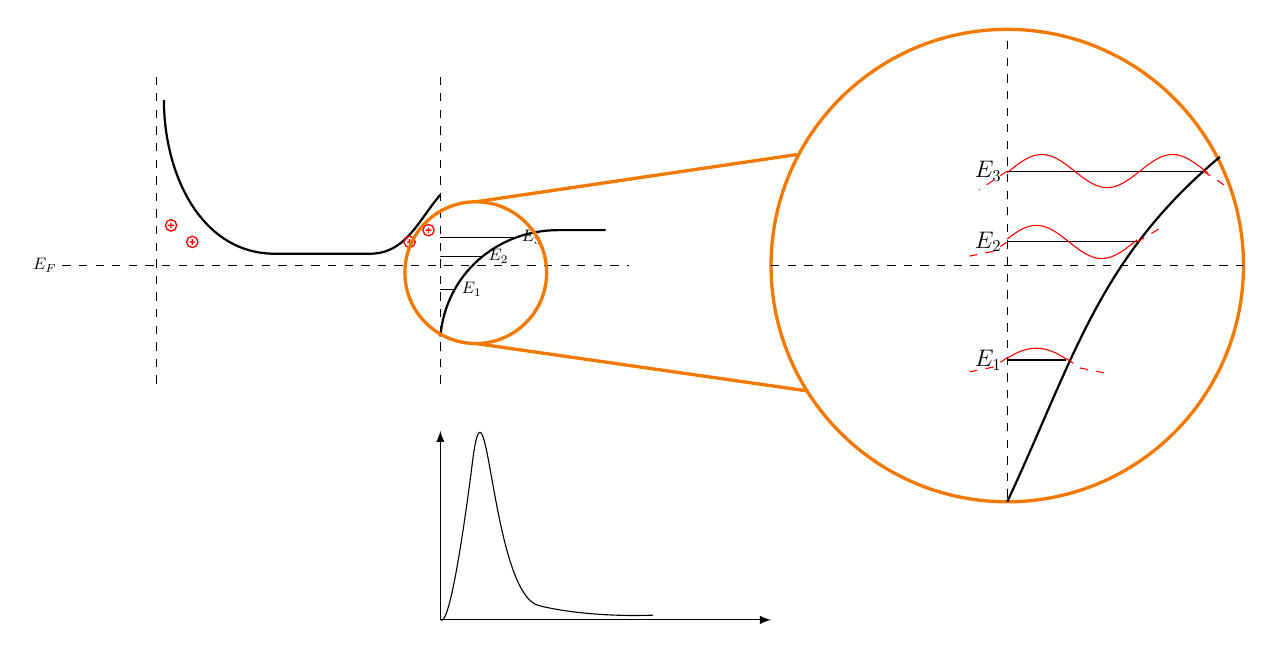
\begin{tikzpicture}[scale=0.6,transform shape]
        \draw[dashed] (0,0) node[left]{$E_F$} -- (12,0);
        \draw[dashed] (2,4) --++ (0,-6.5);
        \draw[dashed] (8,4) --++ (0,-6.5);

        %disegno grafici
        \draw[thick](2.15,3.5) to [in=180, out=270] ( 4.5,0.25)
              --++(2,0)   to [in=230, out=0] ( 8, 1.5 );
              
         \draw[thick](8,-1.5) to [in=180, out=85] ( 10.5,0.75)
              --++(1,0);
        %disegno ioni positivi
        \node at (2.3,0.85) { \tikz\draw [thick,red, scale=0.75]
        circle (0.16cm) (-0.08,0)--(0.08,0) (0,0.08)--(0,-0.08);};
        \node at (2.75,0.5) { \tikz\draw [thick,red, scale=0.75]
        circle (0.16cm) (-0.08,0)--(0.08,0) (0,0.08)--(0,-0.08);};
        \node at (7.75,0.75) { \tikz\draw [thick,red, scale=0.75]
        circle (0.16cm) (-0.08,0)--(0.08,0) (0,0.08)--(0,-0.08);};
        \node at (7.35,0.5) { \tikz\draw [thick,red, scale=0.75]
        circle (0.16cm) (-0.08,0)--(0.08,0) (0,0.08)--(0,-0.08);};
        % disegno livelli energetici
        \draw (8,-0.5)--++(0.33,0)node[right]{$E_1$};
        \draw (8,0.20)--++(0.9,0)node[right]{$E_2$};
        \draw (8,0.60)--++(1.6,0)node[right]{$E_3$};

        %grafico zoom
         \draw[very thick,orange!95!black] (8.75,-0.15) circle (1.5cm);
        % Save coordinates at 90° and 270°
         \coordinate (point90) at (8.75,1.5-0.15);
         \coordinate (point270) at (8.75,-1.5-0.15);
         \draw[very thick,orange!95!black](point90)--++(6.8,1);
         \draw[very thick,orange!95!black](point270)--++(7,-1);
         \draw[very thick,orange!95!black] (20,0) circle (5cm);

         %disegno zoom
         \draw[dashed]  (15,0) --++ (10,0);
         \draw[dashed] (20,4.75) --++ (0,-9.75);
         \draw[thick](8+12,-1.5-3.5) to [in=220, out=65] ( 10.5+14,0.75+1.55);

         %zoom livelli
         \draw (20,-2)node[left]{\Large$ E_1$}--++(1.25,0);
         \draw (20,0.5)node[left]{\Large$E_2$}--++(2.75,0);
         \draw (20,2)node[left]{\Large$E_3$}--++(4.15,0);
         %distribuzione
         \draw[-latex] (8,-7.5) --++ (7,0);
         \draw[latex-] (8,-3.5) --++ (0,-4);
         %disegno concentrazione
         \draw(8,-7.5).. controls (8.25,-7.75) and (8.7,-4)..(8.7,-4);
         \draw(8.7,-4).. controls (9,-2) and (9.1,-7.0)..(10.1,-7.2)..controls (10.1,-7.2) and (11,-7.45).. (12.5,-7.4);
         %plot funzione psi E1
        \draw[red,dashed](20,0.3-2.25)--++(-0.3,-0.2)--++(-0.5,-0.1);
        \draw[red, domain=2:3.25, samples=200, smooth] plot (\x+18, {-2.25+0.5*sin(90*\x+215))});
        \draw[red,dashed](21.25,0.3-2.27)--++(0.3,-0.2)--++(0.5,-0.1);
        %plot funzione psi E2
        \draw[red,dashed](20,0.5)--++(-0.3,-0.2)--++(-0.5,-0.1);
        \draw[red, domain=2:4.75, samples=200, smooth] plot (\x+18, {0.5+0.35*sin(130*\x-250))});
        \draw[red,dashed](22.75,0.5)--++(0.5,+0.3);
        %plot funzione psi E3
         \draw[red,dashed](20,2)--++(-0.3,-0.2)--++(-0.3,-0.2);
        \draw[red, domain=2:6.25, samples=200, smooth] plot (\x+18, {2+0.35*sin(130*\x-265))});
        \draw[red,dashed](24.15,2)--++(+0.3,-0.2)--++(+0.3,-0.2);
    \end{tikzpicture}
    \captionof{figure}{Caption}
    \label{fig:enter-label}
\end{center}

%
Visto che all'elettrone è associata una funzione d'onda e la buca di potenziale non ha pareti infinite, si avrà una situazione in cui la funzione porobabilità $\psi$ esce fuori dalla buca di potenziale.\\
la distribuzione degli elettroni dipenderà dalla probabilità di trovare un elettrone in una particolare posizione, data dal modulo quadro della funzione d'onda ($|\psi|^2$).\\
Quindi, come nel caso MOSFET la distribuzione di carica dei portatori nel canale non è concentrata all'interfaccia ma è del tipo mostrato a sinistra da cui vedo che ha un picco a distanza d dall'interfaccia e non è simmetrica.\\
in generale i livelli al di sotto di $E_F$ sono quelli con la massima probabilità di occupazione.\\
I livello energetici lungo le direzioni y e z hanno un andamento continuo, mentre lungo x l'andamento è discreto. Per questo motivo il gas di elettroni, avendo solo due gradi di libertà continui, viene detto "gas elettronico bidimensionale (2DEG)".\\

\begin{exbox}
    In altre parole, gli elettroni nel canale possono muoversi liberamente nelle direzioni y e z perchè hanno livelli energetici continui. Lungo al direzione x le cariche non sono in moto perchè il potenziale dovuto all'energy gap crea una buca di dimensioni finite creando livelli energetici discreti.
\end{exbox}

Questo tipo di gas elettronico ha alcune importanti caratteristiche:
\begin{enumerate}
    \item Basso rumore perchè ha solo due gradi di libertà (y,z). il rumore termico nel caso tridimensionale ha una densità spettrale pari a $k_BT$, mentre nel caso bidimensionale vale $\frac{2}{3}k_BT$;
    \item Alta mobilità: dovuta al fatto che il canale si crea in un semiconduttore intrinseco (non drogato, cioè con basso $N_D$).
\end{enumerate}
%
\begin{minipage}{0.55\textwidth}
    Non è stato esplicitato prima ma,in questi tipi di transistor, il canale è già formato con $V_G=0$ a causa dei meccanismo fisici e quantistici in gioco. Per chiudere tale canale si deve applicare un potenziale negativo il cui effetto sarà quello di generare un'energia potenziale che alza il livello di fermi intrinseco riducendo la buca di potenziale sopra al livelli di fermi, riducendo la probabilità di occupazione.
    \begin{ricevimento}
        vuoto di memoria. Se Vg negativa. il gate attira ioni positivi oltre a quelli già presenti per la giunzione shottky. ma dall'altra parte
    \end{ricevimento}
\end{minipage}
\hfill
\begin{minipage}{0.4\textwidth}
    \begin{center}
    \begin{tikzpicture}[scale=0.5,transform shape]
        \draw[dashed] (0,0) node[left]{$E_F$} -- (12,0);
        \draw[dashed] (2,4) --++ (0,-4.5);
        \draw[dashed] (8,4) --++ (0,-4.5);

        %disegno grafici
        \draw[thick](2,3.5) to [in=180, out=320] ( 8, 1.5 );
              
         \draw[thick](8,-0.25) to [in=180, out=60] ( 10.5,0.75)
              --++(1,0);
        
        % disegno livelli energetici
        
        \draw (8,0.20)node[left]{$E_2$}--++(0.3,0);
        \draw (8,0.60)node[left]{$E_3$}--++(1,0);
    \end{tikzpicture}
\end{center}
\end{minipage}
\\%
Nel caso di $V_G>0$ il gate si comporta da diodo e comincia a far scorrere corrente, per cui questa situazione va evitata.\\
%
\begin{psbox}
    Ps. questo dispositivo eprmette la ricezione satellitare con antenne a piccolo guadagno
\end{psbox}
%
\cleardoublepage
\subsection{Densità di carica e varianti dell'HEMT}
Nei MOS avevo stabilito che
\begin{equation}
    Q_n^{mos}=-C_{ox}(V_g-V{th})
\end{equation}
in questi oggetti la situazione è più complicata.
suppongo di stabilire la pendenza del diagramma energetico chiamandola Es, dove E= energia, s =slope. allora i livelli energetici della buca di potenziale si possono rappresentare in funzione di questo livello Es:\\
(non serve saperlo)
\begin{equation}
    E_s = \left[\dfrac{3\ h_q\ E_s}{4\sqrt{2\ {m_e}^*}}\left( n+\dfrac{3}{4}\right)\right]^{\dfrac{2}{3}}
\end{equation}

Si vede che dipende dal tipo di semiconduttore e dalla massa efficace. 
La cosa più rilevante è che per capire quanta carica c'è dentro devo fare una consdierazione. ciascuno di questi livelli energetici diventerà un autovaleore della funzione di schrodinger e diventerà un'autofunzione che è alla base della determinazione della probabilità di occupazione di questi livelli energetici.\\(??)
\begin{ricevimento}
    spiegare
\end{ricevimento}

grafico\\
.\\
Quindi si predne l'equazioen di shoredinger per un sistema stazionario che deve essere risolta con l'equazione di poisson:
\begin{align}
    \begin{cases}
        -\dfrac{\hslash^2}{2m_e^*} \, \dfrac{\partial^2 \psi_n}{\partial x^{2}}+E_c(x)\psi_n(x)=E_n \cdot \psi_n(x) \\
        \\
        \dfrac{\partial}{\partial x}\left[ \varepsilon \dfrac{\partial E_c(x)}{\partial x}\right]=q(N_D-n_s)
    \end{cases}
\end{align}
dove $n_s$ è la concentrazione di elettroni all'interno della buca di potenziale formatasi.

\begin{equation}
    n_s=\dfrac{4\pi kTm_e^*}{h^2}\sum_n \left| \psi \right|_n^2 \ln{\left[ 1+e^{\dfrac{E_F-E_n}{k_BT}}\right]}
\end{equation}
Noti $\psi_n$ ed i valori di $E_n$ è possibile determinare una probabilità di occupazione data dalla funzione logaritmo che identifica la probabilità di occupazione rispetto al livello di fermi.\\
chiaramente Ec è incognita. è il profilo di potenziale.

Ora siamo in grado di determinare la distribuzione $\rho$.

Le condizioni a contorno sono due: una a contatto metallo sc e una sc1-sc2

ripeto che tutto questo è un'alìpprossimazione.\\
\begin{ripasso}[roba che non so dove mettere]
    Il problema principale dei FET  èdovuto al fatto che la corrente scorre parallela alla fiunzione di materiali diversi.\\
Le giunzioni di differenti materiali sono caratterizzare dalla creazione di livelli energetici in banda proibita dette trappole che possono intrappolare elettroni e rilasciarli in modo casuale.Questa è l aprincipale sorgente di rumore flicker.\\
Per questo motivo per avere poco rumore flicker si devono usare gli HBT in quanto la corrente scorre perpendicolare alla giunzione ed è quendio meno esposya alle trappole.

\end{ripasso}
ci sono delel varianti che rendono tutto più complicato\\
\paragraph{L'effetto di seconda porta}\mbox{}\\
Io lo chiamo effetto diodo ma Viene comunemente definito come "effetto di seconda porta" o "effetto di gate superiore".\\
\begin{ricevimento}
    cercare l'effetto online per essere sicuri
\end{ricevimento}
%
\begin{minipage}{0.49\textwidth}
    \begin{center}
        \begin{tikzpicture}[scale=0.6, transform shape]
        \draw [white](0,0) rectangle ++ (6,2) node[pos=0.5,black]{$GaAs-i$};
        \draw [dashed](0,2)--++(0,-1);
        \draw [dashed](6,2)--++(0,-1);
        \draw (0,2) rectangle ++ (6,1) node[pos=0.5]{$Al_{0.3}Ga_{0.7}A_s-n^+$};

        %metalizzazioni
        \draw[pattern = north east lines, pattern color = black] (2,3) rectangle ++(2,0.25);
        \draw(+3,3.25)to[short,-*]++(0,0.2) node[right]{G};
        
        \draw[pattern = north east lines, pattern color = black] (0,1.5) rectangle ++(-0.2,1) ;
        \draw(-0.2,2)to[short,-*]++(-0.2,0) node[left]{S};
        
        \draw[pattern = north east lines, pattern color = black] (6,1.5) rectangle ++(+0.2,1);
        \draw(+6.2,2)to[short,-*]++(+0.2,0) node[right]{D};
        %disegno lacune
        \foreach \pos in {0.75,1.5,2.25,...,5.5} {
        \node at (\pos,2.2) { \tikz\draw [thick,red, scale=0.75]
        circle (0.16cm) (-0.08,0)--(0.08,0) (0,0.08)--(0,-0.08) ;} ;}
        %disegno elettroni
        \foreach \pos in {0.5,1,1.5,2,...,5.5} {
         \node at (\pos,1.8) { \tikz\draw [thick,fill=Ecolour]
        circle (0.13cm) (-0.08,0)--(0.08,0) ;};}
    \end{tikzpicture}
    \captionof{figure}{Caption}
    \end{center}
\end{minipage}
\hfill
\begin{minipage}{0.49\textwidth}
       \begin{center}
        \begin{tikzpicture}[scale=0.6, transform shape]
        \draw [white](0,0) rectangle ++ (6,2) node[pos=0.5,black]{$GaAs-i$};
        \draw [dashed](0,2)--++(0,-1);
        \draw [dashed](6,2)--++(0,-1);
        \draw (0,2) rectangle ++ (6,0.25) node[pos=0.5]{\tiny $Al_{0.3}Ga_{0.7}A_s-n^+$};
        \draw (0,2.25) rectangle ++ (6,1) node[pos=0.5]{$Al_{0.3}Ga_{0.7}A_s-i$};

        %metalizzazioni
        \draw[pattern = north east lines, pattern color = black] (2,3.25) rectangle ++(2,0.25);
        \draw(+3,3.5)to[short,-*]++(0,0.2) node[right]{G};
        
        \draw[pattern = north east lines, pattern color = black] (0,1.5+0.125) rectangle ++(-0.2,1) ;
        \draw(-0.2,2+0.125)to[short,-*]++(-0.2,0) node[left]{S};
        
        \draw[pattern = north east lines, pattern color = black] (6,1.5+0.125) rectangle ++(+0.2,1);
        \draw(+6.2,2+0.125)to[short,-*]++(+0.2,0) node[right]{D};
        %disegno lacune
        \foreach \pos in {0.75,2.25,...,5.5} {
        \node at (\pos,2.45) { \tikz\draw [thick,red, scale=0.75]
        circle (0.16cm) (-0.08,0)--(0.08,0) (0,0.08)--(0,-0.08) ;} ;}
        %disegno elettroni
        \foreach \pos in {0.5,1,1.5,2,...,5.5} {
         \node at (\pos,1.8) { \tikz\draw [thick,fill=Ecolour]
        circle (0.13cm) (-0.08,0)--(0.08,0) ;};}
    \end{tikzpicture}
    \captionof{figure}{Caption}
    \end{center}
\end{minipage}

Negli HEMT la mobilità aumenta perchè gli elettroni entrano in un semiconduttore intrinseco però c'è da fare i conti con gli ioni fissi che lasciano dietro di loro quando "saltano dentro questo semiconduttore". 
Il fenomeno è simile a quello che accadrebbe nel caso di polarizzazzione positiva ($V_g>0$), dove il canale si riempie di lacune. Allo stesso modo, l'accumulo di carica fissa positiva può creare una regione (di svuotamento) come fosse un diodo portando a una maggiore corrente di leakage o a una modulazione indesiderata del comportamento del dispositivo HEMT.

L'uso dello strato spacer è una delle tecniche utilizzate per mitigare questi effetti. Lo strato spacer aiuta a separare gli ioni positivi dalla regione di interesse. Lo spessore dello spacer deve essere sottile per non interferire con l'iniezione degli elettroni nel canale, ma anche spesso per allontanare gli ioni, va quindi ottimizzato.\\

si ottiene la struttura chamata HEMT pseudomorfico.

\begin{figure}[hbt!]
    \centering
    \begin{circuitikz}
        \draw (0,0) rectangle ++ (6,1.5) node[pos=0.5]{$GaAs-i \ \ \  BUFFER$};
        \draw (0,1.5) rectangle ++ (6,2) node[pos=0.5]{$GaAs-i$};
        \draw (0,3.5) rectangle ++ (6,0.5) node[pos=0.5]{\scriptsize{$Al_{0.3}Ga_{0.7}As-i$}};
        \draw (0,4) rectangle ++ (6,0.75) node[pos=0.5]{$Al_{0.3}Ga_{0.7}As-n^+$};
        
        %metalizzazioni
        
        \draw[pattern = north east lines, pattern color = black] (2,4.75) rectangle ++(2,0.25);
        \draw(+3,5)to[short,-*]++(0,0.2) node[right]{G};

        %disegno i tratteggi per il diagramma a bande
        \draw[densely dotted] (9,0)--++(6,0);
        \draw[densely dotted] (9,1.5)--++(6,0);
        \draw[densely dotted] (9,3.5)--++(6,0);
        \draw[densely dotted] (9,4)--++(6,0);
        \draw[densely dotted] (9,4.75)--++(6,0);
        
        \draw[densely dotted] (12,5)--++(0,-5.5)node[anchor=north]{\footnotesize{Ef}};
        \draw[densely dotted] (13.75,0)--++(0,-0.5)node[anchor=north]{\footnotesize{Ec}};
        \draw[<->](12,0)--(13.75,0) ;
        \node at (12.95,0)[below]{\footnotesize{$\dfrac{E_g}{2}$}};
        
        % disegno diagramma a bande 
        \draw(15,4.75) to [in=155, out=181,distance=1cm](14,4); 

        \draw(10.5,4) to [in=90, out=340](11,3.5);
        
        \draw(12.5,3.5) to [in=90, out=340](13.75,0);

        %disegno cariche positive
        \foreach \pos in {0.5,1,1.5} {
        \node at (12.25+\pos,4.65) { \tikz\draw [thick,red, scale=0.7]
        circle (0.10cm) (-0.05,0)--(0.05,0) (0,0.05)--(0,-0.05) ;} ;}
        
        \foreach \pos in {0.5,1,1.5,2,2.5,3} {
        \node at (10.5+\pos,4.1) { \tikz\draw [thick,red, scale=0.7]
        circle (0.10cm) (-0.05,0)--(0.05,0) (0,0.05)--(0,-0.05) ;} ;}
        
        %disegno cariche negative
        \node at (14,4.25) { \tikz\draw [thick,blue, scale=1.25]
        (-0.05,0)--(0.05,0);};
        % label
        \draw[|-|](12,4.75)node[anchor=south west]{$qV_{bi}$}--++(3,0) ;
    \end{circuitikz}
    \caption{Caption}%
    \label{fig:enter-label}
\end{figure}
\begin{tikzpicture}[overlay]
          %frecce label
        \draw[](7.75,4.375+3.25)node[blue]{Cap layer};
        \draw[](7.75,4.375+2.5)node[blue]{Supply layer};
        \draw[](7.75,3+3.25)node[blue]{Space layer};
        \draw[](7.75,2.5+2.5)node[blue]{Channel layer};
        \draw[](7.75,0.75+2.5)node[blue]{Substrate};
        
    \end{tikzpicture}
 il pHEMT che si verrà ad ottenere avrà un canale, detto quantum well, a forma per lo più rettangolare, al contrario del classico HEMT in Figura \ref{fig:Struttura di un HEMT} che assume un canale a forma triangolare.
\subsubsection{Pseudomorfic HEMT: p-HEMT}
\noindent\begin{minipage}{0.6\textwidth}
    Il poblema dell'HEMT è che la carica confinata in modo quantistico all'interno del canale 2DEG può essere bassa in quanto la buca che li occupa può essere piccola. Se si osserva l'andamento della velocità media $v_d$ in relazione dal campo elettrico $\mathcal{E}$ ( eq uindi la mobilità), si vede che esiste il composto InGaAs che presenta una mobilità molto elevata per $\mathcal{E}$ bassi.
\end{minipage}
\hfill
\begin{minipage}{0.3\textwidth}\raggedleft
    \begin{center}
    \includegraphics[width=1\textwidth]{Immagini/imm27.11.2023/mobilità materiali.png}
\end{center}
\end{minipage}
%
\noindent\begin{minipage}{0.6\textwidth}
Inoltre come si osserva dal grafico a destra si avrà che il passo reticolare dell'InGaAs è simile a quello dell'AlGaAs, ma presentano due $E_g$ molto diversi. Maggiore è la funzione reticolare x dell'indio e minore sarà l'energy gap. Essendo quindi InGaAs costruito per avere una struttura con $E_g$ minore rispetto alle altre alternative, si avrà aumento della dimensione della sezione del canale rettangolare creando maggior numero di livelli discreti disponibili nella buca e quindi aumentando la carica disponibile al trasporto (se $\nabla E_g^{InGaAs} \downarrow$ allora $\nabla E_g \uparrow$). 

\end{minipage}
\hfill
\begin{minipage}{0.3\textwidth}\raggedright
\begin{center}
    \includegraphics[width=1\textwidth]{Immagini/imm27.11.2023/speudomorfic materiali.png}
    \end{center}
\end{minipage}
\\%
Il motivo di questa differenza nella dimensione del quantum well si speiga proprio dal fatto che l'energia ($E_g$) necessaria per passare dalla una banda di valenza a quella di conduzione è bassa, comportando che gli elettroni possono superare la barriera energetica più facilmente e consentendo la formazione di un quantum well più ampio senza rischio significativo di emissione spontanea cioè con meno probabilità che gli elettroni vengano "sparati" fuori dalla regione del quantum well a causa dell'energia termica.
La struttura spiegata è la seguente:

\begin{figure}[hbt!]
    \centering
    \begin{tikzpicture}
        \draw(0,0)rectangle++(2,1);
        \draw(0,1)rectangle++(2,1);
        \draw(0,2)rectangle++(2,1);

        \draw(0.5+3,0)--++(0,1)--++(0.25,0)--++(0,1)--++(-0.75,0)--++(0,1);
        \draw(1.5+3,0)--++(0,1)--++(-0.25,0)--++(0,1)--++(+0.75,0)--++(0,1);
        %disegno realistico
        %energia di fermi
        \draw(7.5,0)--++(0,4);
        % disegno diagramma a bande 
        \draw(9.5,3) to [in=155, out=181,distance=1cm](8.75,2)--(6.5,2); 

        \draw(6.5,2) to [in=90, out=340](7.25,1)--++(0.75,0);
        
        \draw(8,1) to [in=90, out=340](8.75,0);
    \end{tikzpicture}
    \caption{Caption}%
    \label{fig:enter-label}
\end{figure}

Quindi il vantaggio della struttura InGaAs è principalmente quello di avere un canale più grande, consentendo tanta più carica disponibile ed una migliore mobilità dei portatori, con tutte le dirette conseguenze.
L'insieme di questi aspetti creano una versione dell'HEMT molto vantaggiosa ma ovviamente ci sono delle limitazioni realizzative. Ricordo che stò parlando di semiconduttori con passo reticoare differente,quindi , non posso muovermi tanto dal passo reticolare 0.5 di GaAs perchè altrimenti rischiod i avere disclocazioni.
Allora quello che succede è che entra in gioco uno spessore "spessore critico" del materiale che dev'essere opportunamente definito perchè altrimenti si creano difetti reticolari ed il disppositivo non funziona bene.
è detto spessore critico o pseudomorfo e in funzione della funzione molare definisce qual'è lo spessore del materiale posto che ci siano un valore massimo di dislocazioni accettabili.
se si ammette un 2\% di dislocazioni alloralo spessore critico diventa infinito se x=0 però poi asume valori anche molto piccoli per frazioni molari dell'ordine dello 0.5
grafico\\

\begin{exbox}[dove emttere?]
Ritornano ancora al pHEMT InGaAs. Le bande sono tali che una volta tolti i salti dovuti ai diversi $E_g$ risulti un profilo continuo.\\
Se si usa uno strato di InGaAs ad alta concentrazione di In si ottengono $E_g$ piccoli, per cui si aumenta la profonditò della quantum well, ma come si vede dal grafico a destra si riduce lo spessore critico realizzabile.
\end{exbox}
\begin{figure}[hbt!]
    \centering
    \begin{tikzpicture}
        %disegno asse x
        \draw[-latex](0,0)--++(5,0)node[right]{$x$};
        %disegno asse y
        \draw[-latex]((0,0)--++(0,5)node[left]{$t_c$};
        %disegno grafici
        \draw(0.2,4.5) ..controls (0.2,0.5) and (1.5,0.05).. (4.5,0.05);
        %label
        \draw[dashed](0,0.35)node[left]{$70$}--++(2,0) %
                      (2,0)node[below]{$0.5$}--++(0,0.35);
        \draw[dashed](0,0.76)node[left]{$100$}--++(1.25,0) %
                      (1.25,0)node[below]{$0.3$}--++(0,0.76);
        \draw[dashed](0,2.05)node[left]{$400$}--++(0.5,0) %
                      (0.5,0)node[below]{$0.1$}--++(0,2.05);
    \end{tikzpicture}
    \caption{Caption}%
    \label{fig:enter-label}
\end{figure}
\subsubsection{Controllo di carica di un P-HEMT}
grafici pg 27.\\
Si vuole trovare la quantità di carica immagazzinata nel canale. per fare questo si deve risolvere l'equazione si Schroedinger lungo il profilo della quantum well.\\
la carica avrà un picco nella zona centrale del supply layer visto che ai lati si hanno ioni positivi, inoltre si avrà un picco nel channel layer dovuto agli elettroni che si spostano nella quantum well. Se si applica un potenziale negativo si può arrivare alla condizione in cui la carica nel supply layer $n_{SL}$ è circa nulla.\\
Si applica la legge di Poisson alla struttura e si trova che:
\begin{equation}
    \varepsilon \dfrac{\partial^2V(x)}{\partial x^2}=q(N_D(x)-n(x))
\end{equation}
La $V(x)$ dell'equazione di Poisson è la $V_C(x)$ del mio problmea ma privo della discontinuità lungo x. Quindi per risolvere il mio problema devo inserire questa discontinuità del potenziale prima di mettere tutto dentro l'equazione di shrodinger. Devo inserire dentro V(x) le condizioni a contorno, ottenendo:

\begin{equation}
    \dfrac{E_C(x)}{q}=V(x)+\Delta E_{C1}(x-x_1)+\Delta E_{C2}(x-x_2)
\end{equation}
dove $E_C(x)=qV_C(x)$ è il profilo della banda del p-HEMT.
Questo formula si deve inserire all'interno dell'equazione di schoedinger per trovare i livelli energetici En nell quantum well.\\
\begin{equation}
    schoedinger equation
\end{equation}
Poi considero le condizioni al contorno
\begin{equation}
    \begin{cases}
        V_C(x=0)=V_{bi}-V_g\\
        V_C(x\rightarrow \infty)=\dfrac{E_g}{2q}
    \end{cases}
\end{equation}

Andando a risolvere questo sistema in modo approssimato si trova che :
\begin{equation}
    E_n=\left[\dfrac{3hqE_s}{4\sqrt{2m_e^*}}(n+\dfrac{3}{4})\right]^{\frac{2}{3}}
\end{equation}
-


con Es derivata nel punto blu.
\begin{equation}
   n_{2DEG}=\dfrac{4\pi kTm_e^*}{h^2}\sum_n \left| \psi \right|_n^2 \ln{\left[ 1+e^{\dfrac{E_F-E_n}{k_BT}}\right]}
\end{equation}
Si ha per $n_{2deg}$ il rpodotto tra una probabilità di occupazione e una funzione di distribuzione che dipende dalll distanza tra il livello n-esimo di $E_F$, per cui dipende anche da $V_G$.\\
Per valori di $V_G$ abbastanza alti e negativi si può dire che $n_{2deg}$ è proporzionale a $V_G$ (l'esponenziale prevale su 1 dentro al logaritmo).\\
Nel caso in cui la carica $n_{sc}$ si in pinch-off, ovvero $n_{sc} \approx 0$, si può scrivere la carica dentro al canale $n_{2deg}$ come fosse quello in un MOSFET:
\begin{equation}
    n_{2deg}=\dfrac{\varepsilon}{d_{sc}+\Delta d}(V_G-V_{yh})
\end{equation}
In cui $V_{th}=\frac{\phi_{bi}-\nabla E_C}{q}-\frac{qN_D d_{sc}^2}{2\varepsilon}$ è negativo e $V_G-V_{th}$ è positivo.\\
Questa approssimazione permette di calcolare la corrente $I_{DS}$ nel caso di canale corto come si faceva per un mosfet:
\begin{equation}
    I_{DS}=\dfrac{\varepsilon v_{sat} W}{d_{sc}+\Delta d}(V_G-V_{th})
\end{equation}
Il circuito equivalente di un HEMT è simile a quello di un MOSFET.

----------------------\\
Efficienza di modulazione del canale
1)supply layer. aumento $V_G<0$per andare in pinch off $n_{sl}$
2)ma tutto il 2DEG và a $v_{sat}$

poichè quello che trovo è...\\
-------------------\\
\cleardoublepage
\subsubsection{Condizioni di non idealità di un HEMT}
Le principali non idealità dell'HEMT sono due e porteranno a queste conclusioni:
\begin{enumerate}
    \item nel supply layer ho bisogno di avere una polarizzazione negativa per chiudere il canale parassita  e quindi per mandare in pinchoff il FET parassita;
    \item non tutte le cariche nel canale 2DEG si muovono a velocità di saturazione.
\end{enumerate}
\subsubsection{FET parassita nel supply layer}
Con il paragrafo precedente ho ottenuto l'andamento delle cariche all'interno del canale e si può studiare come esso varia al variare delle caratteristiche e della polarizzazione.\\
E' importante notare le differenze che si possono ottere a seconda dei dispositivi in uso. A seguire mostrerò la differenze dell'andament di carica nel canale fra la struttura AlGaAs/InGaAs/GaAs e la struttura AlGaAs/GaAs, nel caso di polarizzazione $V_G \geq 0$ e $V_G<0$.\\
Nel grafico a sinistra ho identificato con il punto $x_1$ la giunzione tra supply layer e space layer mente il punto $x_2$ è il punto di giunzione tra supply layer e channel layer.\\
Nel grafico a destra ho identificato con il punto $x_1$ la giunzione tra supply layer e channel layer.\\
%
\noindent\begin{minipage}{0.4\textwidth}
    \begin{center}
    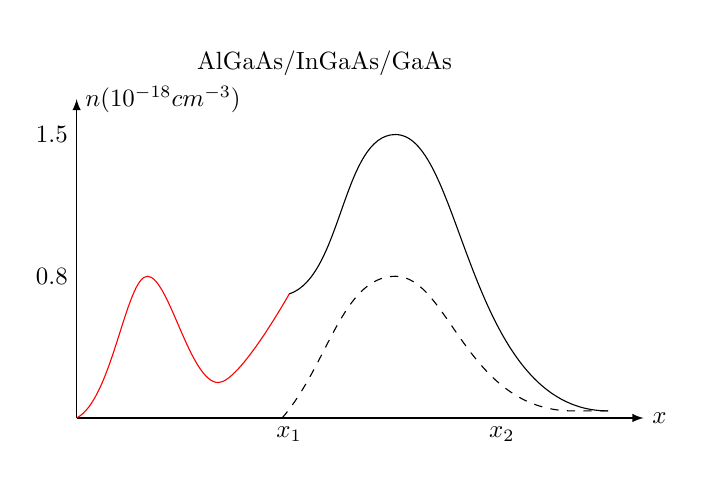
\begin{tikzpicture}[scale=0.9,transform shape]
        %scrivo nome struttura
        \draw[white](0,4.5)rectangle(7,5.5)node[pos=.5,black]{AlGaAs/InGaAs/GaAs};
         %disegno asse x
        \draw[-latex](0,0)--(8,0)node[right]{$x$};
        %disegno asse y
        \draw[latex-](0,4.5)node[right]{$n(10^{-18}cm^{-3})$}--(0,0);
        %label su asse y ed x
        \node at (0,2)[left]{$0.8$};
        \node at (0,4)[left]{$1.5$};
        
        \node at (3,0)[below]{$x_1$};
        \node at (6,0)[below]{$x_2$};
        
        %disegno nsl
        \draw[red](0,0)..controls (0.5,0.25)and(0.7,2)   ..(1,2)  
                       ..controls (1.3,2)   and(1.6,0.5) ..(2,0.5)  
                       ..controls (2.3,0.5) and(3,1.75)  ..(3,1.75);
                
        %disegno 2DEG
        \draw (3,1.75)..controls (3.75,2)and(3.75,4)..(4.5,4)  
                      ..controls (5.45,4)and(5.5,0.1)..(7.5,0.1);
                      
        %disegno 2DEG tratteggiato
        \draw[dashed] (2.9,0)..controls (3.55,0.75)and(3.75,2)..(4.5,2)  
                      ..controls (5.25,2)and(5.5,0.1)..(7,0.1)--++(0.5,0);
        
    \end{tikzpicture}
    \captionof{figure}{Caption}
    \label{fig:enter-label}
\end{center}
\end{minipage}
\hfill
\begin{minipage}{0.5\textwidth}\raggedleft
    \begin{center}
    \begin{tikzpicture}[scale=0.9,transform shape]
        %scrivo nome struttura
        \draw[white](0,4.5)rectangle(7.5,5.5)node[pos=.5,black]{AlGaAs/GaAs};
         %disegno asse x
        \draw[-latex](0,0)--(8,0)node[right]{$x$};
        %disegno asse y
        \draw[latex-](0,4.5)node[right]{$n(10^{-18}cm^{-3})$}--(0,0);
        %label su asse y ed x
        \node at (0,2)[left]{$0.8$};
        \node at (0,4)[left]{$1.5$};
        
        \node at (3,0)[below]{$x_1$};
    
        
        %disegno nsl
        \draw[red](0,0)..controls (0.9,0.5)and(1,1.25)   ..(1.5,1.25)  
                       ..controls (2,1.25)   and(2.5,0.2) ..(3,0.6) ;
                
        %disegno 2DEG
        \draw (3,0.6)..controls (3.75,1)and(3.75,2)..(4.35,2)  
                      ..controls (5.15,2)and(5.5,0.1)..(7.5,0.1);
                      
        %disegno 2DEG tratteggiato
        \draw[dashed] (3,0)..controls (3.7,0.5)and(3.75,1.5)..(4.35,1.5)  
                      ..controls (5.15,1.5)and(5.5,0.1)..(7,0.1)--++(0.5,0);
        
    \end{tikzpicture}
    \captionof{figure}{Caption}
    \label{fig:enter-label}
\end{center}
\end{minipage}
\\%
Nella prima struttura:
\begin{itemize}
    \item Polarizzando il gate con $V_G \geq 0 $ si inietta una certa quantità di carica dentro il canale fino ad un picco di circa $n=1.5 \cdot 10^{-18}/cm^-3$;
    \item Nel punto $x_1$ il valore di n è circa la metà del picco.
\end{itemize}
Nella seconda struttura:
\begin{itemize}
    \item Polarizzando il gate con $V_G \geq 0 $ si inietta una certa quantità di carica dentro il canale fino ad un picco di circa $n=0.8 \cdot 10^{-18}/cm^-3$;
    \item Nel punto $x_1$, cioè nel punto di giunzione tra i due semiconduttori, il valore di n è circa la metà del picco.
\end{itemize}

In entrambi i casi si nota la presenza di un'incurvatura prima di $x_1$ che non esisterebbe nel caso ideale.
Succede che in entrambe le situazioni, quando i gate è polarizzato positivamente o comunque prossimo allo zero, esiste un canale di elettroni parassiti all' interno dell' $ALGaAs$ causato dall'accumulo degli ioni positivi tra le giunzioni.\\
Ho visto ad inizio capitolo il diagramma a bande dell'HEMT ed ho parlato di ioni fissi positivi che si formano tra la giunzione Metallo-semiconduttore e la giunzione supply layer-channel layer. l'ultimo tassello del puzzle è quello di considerare che gli ioni non occupano tutto lo spazio ma lasciano nello strato più interno un canale grande abbastanza per il trasporto di elettroni mobili parallelo a quelli che si muovono nel channel layer. Peccato che il canale abbia una bassa efficienza(mobilità scarsa)

\begin{figure}[hbt!]
    \centering
    \begin{tikzpicture}
        %disegnosubstrato e cariche
        \draw(0,5)rectangle(9,6)node[pos=0.5]{GaAs};
        \draw(0,6)rectangle(9,7);
        
        \begin{scope}[scale=0.5,transform shape]
             %disegno lacune Me-SC
            \draw[densely dotted](0,14)rectangle++(18,-0.75);
            \foreach \pos in {0.75,1.5,2.25,...,7} {
            \node at (\pos+5.2,13.65) { \tikz\draw [thick,red, scale=0.75]
            circle (0.16cm) (-0.08,0)--(0.08,0) (0,0.08)--(0,-0.08) ;} ;}
            %disegno elettroni
            \foreach \pos in {1,2,3,...,11} {
             \node at (\pos+3,13) { \tikz\draw [thick,fill=Ecolour]
            circle (0.1cm) (-0.08,0)--(0.08,0) ;};}
            %disegno lacune SC1-SC2
            \draw[densely dotted](0,12)rectangle++(18,0.75);
            \foreach \pos in {0.75,1.5,2.25,...,12} {
            \node at (\pos+2.65,12.35) { \tikz\draw [thick,red, scale=0.75]
            circle (0.16cm) (-0.08,0)--(0.08,0) (0,0.08)--(0,-0.08) ;} ;}
        \end{scope}
        
        \draw[fill=white] (0,6.9)--(0,5)--(1,5) to[in=290, out=70] (1,7) ;
        \draw[fill=white] (9,5.1)--(9,7)--(8,7) to[in=115, out=245] (8,5);

        
        %metallizzazioni
        \draw[fill=gray](0.25,7) rectangle++(0.5,0.125)
        (0.5,7.125)--++(0,0.25) node[anchor=south]{S};
        \draw[fill=gray](3,7) rectangle++(3,0.125)
        (4.5,7.125)--++(0,0.25) node[anchor=south]{G};

        \draw[fill=gray](8.25,7) rectangle++(0.5,0.125)
        (8.5,7.125)--++(0,0.25) node[anchor=south]{D};

        \draw[latex-,cyan](2.5,5.75)--(6.5,5.75)node[right]{$I_{ch}$};
        \draw[latex-,blue](6.6,6.57)--(7.2,6.57)node[right]{$I_{sl}$};

    \end{tikzpicture}
    \caption{Caption}%
    \label{fig:enter-label}
\end{figure}

Quindi, per entrambi i dispositivi, in casi di potenziale sufficientemente alto o comunque intorno allo zero, sotto il contatto di gate, non è detto che tutta la parte SC  sia svuotata ma magari può ancora avere uno strato interno in cui c'è carica mobile.\\ si crea un rigurgito della carica che può raggiungere anche livelli sufficientemente alti.\\
--------------------------\\
La prima struttura è costituita da elettroni in una è del bulck l'altra è del 2deg
e c'è differenza tra le due . questi elettroni  sopra si muovonno in un canale fet tradizionale  mentre quegli altri nel gas .le differneze tra gli ordini di grandezza delle mobilità è notevole.\\
-----------------------------\\

L'effetto presentato sopra descrive esattamento il comportamento di un transistor a effetto campo. Il problema è che questo  FET è un fenomeno parassita e quindi è opportuno cercare di minimizzarlo. La soluzione al problema è quello di mandare il fet parassita in pinch off applicando una $V_G < 0$ in modo che $n_sl$ ed $n_{bulk}$ siano circa 0 ma mantenendo $n_{2DEG} \neq 0$. \\
%
Questa è l'unica soluzione. L'alternativa sarebbe convivere con due transistor, uno HEMT con buone prestazioni  e l'altro FET con pessime prestazione, poste in parallelo tra loro comportando un generale abbassamento della qualità del dispositivo.\\
%
la cosa fondamentale è che il 2deg ha un picco di corrente di carica due volte maggiore del classico HEMT però entrambi si portano dietro l'eccesso di carica del supply layer. Questo spiega anche perchè questi transistor funzionao meglio quando c'è meno carica iniettata al gate, per avere meno contributi di carica in eccesso dal supply layer.
%
\subsubsection{altre non idealità}
    un altro fenomeno che si innesca in questi dipositivi è legato al fatto che funzionano con elevati campi elettrici nel canale.\\
    Gli elettroni mobili in una zona ad elevato campo elettrico si muoveranno praticamente alla velocità di saturazione, comportando la saturazione della corrente.\\
    La saturazione della corrente è causata per lo più dalla saturazione della velocità mentre il pinchOFF ha un impatto minore. In particolare:
    \begin{enumerate}
        \item Nei MOSFET a canale corto, la saturazione della corrente avviene per la velocità delle cariche
        \item Nei MOSFET a canale lungo, la saturazione della corrente si ha per il pinchOFF
    \end{enumerate}
\begin{psbox}[INFO consigliato sapere]
    La differenza tra saturazione della corrente dovuta a strozzatura del canale (pinch off) o saturazione della velocità?\\

    Nei materiali come il silicio, che è comunemente usato nei transistor MOSFET, raggiunta una certa intensità di campo elettrico, la velocità degli elettroni raggiunge un massimo. Oltre questo punto, anche se applichi un campo elettrico più elevato, gli elettroni non possono accelerare ulteriormente. Questo è noto come saturazione della velocità.\\

    Nel MOSFET, il canale tra source e drain è controllato dalla tensione di gate. Quando la tensione di gate supera una certa soglia, il canale si chiude, e questo è noto come pinch-off o strozzatura del canale. Quando il canale è chiuso, la corrente attraverso il MOSFET è massima e indipendente dalla tensione di drain. Il valore della corrente è data dalla legge di continuità.

    il pinch off ha una saturazione di corrrente che cambia con la tensione di gate mentre la saturazione di velocità dipende dal campo elettrico cioè da "Vd/W = Vd/lunghezza del canale"
\end{psbox}

ci interessa capire che in realtà il dispositivo non è del tutto saturo.\\

\paragraph{Frequenza di taglio}\mbox{}\\
poichè il campo elettrico $\mathcal{E}$ non è costante lungo tutto il canale, solo alcune cariche viaggiano a $v_d^{dat}$, quindi in totale abbiamo due fenomeni non ideali che degradano le prestazioni del transistor:
\begin{enumerate}
    \item FET parassita: è necessario aumentare la tensione negativa di gate per mandare in pinch off il JFET.
    \item Incoerenza della velocità del gas bidimensionale.non è vero che tutti gli elettroni si muovano dentro al canale a $v_{sat}$ perchè non è vero che il campo elettrico è costante su tutto il canale. ma è maggiore vicino al drain e diminuisce verso il source (nel caso $V_{DS}>0$).\\
\end{enumerate}
la combinazione di questi due fenomeni osservati sperimentalmente ha portato a capire come la frequenza di taglio ft non è costante ma si riduce.\\
Ricordo la formula della frequenza di transizione $f_t$:
\begin{equation}
    f_t=\dfrac{g_m}{2\pi C_{gs}}
\end{equation}
tramite manipolazione matematica posso riscriverlo come:
\begin{equation}
    f_t=\dfrac{g_m}{2\pi C_{gs}}\cdot \color{red}\dfrac{v_{gs}}{v_{gs}} \color{black}=\dfrac{\partial I_{drain}}{2\pi \partial Q_{gate}}=\dfrac{\partial \dfrac{ Q_{sat}}{L_gv_{sat}}}{2\pi \partial Q_{gate}}=\dfrac{v_{sat}}{2\pi L_g}\cdot\left[ \dfrac{\partial Q_{sat}}{\partial Q_{gate}}\right]
\end{equation}
dove:
\begin{itemize}
    \item $gm \cdot v_{gs}$ è il differenziale della corrente di drain
    \item $C_{gs} \cdot v_{gs}$ è il differenziale della carica di gate
\end{itemize}
se la corrente di drain deve essere la corrente che viaggia a velocità saturata, allora Idrain sarà differenziale di carica/tempo di transito cove il tempo di transit è la lunghezza di gate/velocità saturata.\\

tutto questo si traduce in una $f_t$ per piccoli segnali pari a:
\begin{equation}
    f_t=\dfrac{v_{sat}}{2\pi L_g}\cdot\left[ \dfrac{\partial Q_{sat}}{\partial Q_{gate}}\right]
\end{equation}
dove $L_g/V_{sat}= tempo di transito$.\\
se $\dfrac{\partial Q_{sat}}{\partial Q_{gate}}$ fosse 1 allora sarebbe tutto apposto, le cariche si muoverebbero a velocità saturata, peccato che non è mai 1. Nella realtà la carica che viaggia a velocità saturata è minore della carica totale che vede il gate.\\


Si osserva l'andamento della banda di conduzione nelle sezioni AA'sotto al metallo e BB'. Si osserva come si adentro al supply layer, sia dentro al substrato la zona che può ospitare carica diventi più grande se non è sotto il metallo.\\
si avrà quindi che la zona esterna può ospitare una quantità maggiore di carica rispetto alla zona sotto al gate.\\
inoltre se si applica il potenziale $V_D$ come in figura l'andamento della carica nel canale assumerà la forma disegnata. Quindi in pratica se il campo elettrico sotto al gate è molto intenso si può dire che solo le cariche nella zona blu sono quelle che si spostano a $v_{sat}$, mentre le altre si muoveranno a velocità inferiore in modo da mantene la corrente costante.\\
L'effetto di queste due non idealità di ritrovano nel calcolo della frequenza di transizione. Questa infatti risulta sovrastimata se calcolata con formula:



Infatti la $f_t$ può essere misurata a partire dai parametri S, misurati per alcuni specifici di frequenza, che vanno convertiti in parametri H.\\
Interpolando linearmente le misure del parametro $h_{21}$ si trova $f_t$ quando arriva ad essere 0dB.\\
Si moltiplica e divide $f_t$ per $v_{gs}$:
le ee rimaste.\\
\paragraph{Efficenza di modulazione}\mbox{}\\
Si può definire l'efficienza di modulazione:
\begin{equation}
    ME=\dfrac{dQ_{sat}}{dQ_{gate}}
\end{equation}
che è una quantità minore di 1 visto che la carica a $v_{sat}$ è solo una parte di quella sotto al gate.\\
L'efficenza di modulazione si può vedere come divisa in due parti: una dipendente dalla carica nel canale 2DEG che si muove a $v_{sat}$ e l'altra dipende dalla carica nel supply layer $\text{ME}_\text{sl}$ che si muove a velocità diversa da $v_{sat}$.\\
Il primo si può trovare con la formula:
\begin{equation}
    ME_{sl}=\dfrac{dn_{2DEG}}{dn_{2DEG}+dn_{sl}}
\end{equation}
\begin{figure}[hbt!]
    \centering
    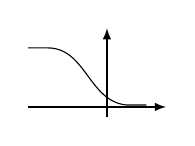
\begin{tikzpicture}[scale=0.25]
        %disegno asse x
        \draw[-latex](-4,0)--(3,0);
        %disegno asse y
        \draw[latex-](0,4)--(0,-0.5);
        %disegno ME_sl
        \draw (-4,3)--++(1,0) to [out=0, in=175](1,0.1)--++(1,0);
        
    \end{tikzpicture}
    \caption{Caption}%
    \label{fig:enter-label}
\end{figure}
\\%
il secondo invece dipende dalla giunzioen schottky che si forma nei contatti di source e drain:
\begin{equation}
    ME_{sat}=\dfrac{dQ_{sat}}{d(Q_{sat}+Q_{GC}+Qn_{sl})}=\dfrac{n_{sat}}{n_{2DEG}}
\end{equation}
La quantità di carica che viaggia a $v_{sat}$ tra tutta quella sotto al gate aumenta all'aumentare di $V_G$.\\
L'andamento cumulativo di ME sarà quindi il prodotto tra i due come nel grafico. si avrà un ME con un massimo per il valore di $V_G$ poco minore di 0. Questo significa che per avere $f_t$ massima sideve lavorare con $V_G$ di qeusto tipo- per lo stesso valore di $V_G$ si ha anche il massimo valore di $G_m$
\begin{figure}[hbt!]
    \centering
    \begin{tikzpicture}
%disegnosubstrato
        \draw(0,5)rectangle(9,6.5)node[pos=.5]{$GaAs_i$};
        \draw(0,6.5)rectangle(9,7)node[pos=.5]{$AlGaAs_n$};
        \draw[fill=white] (0,6.9)--(0,5)--(1,5) to[in=290, out=70] (1,7) ;
        \draw[fill=white] (9,5.1)--(9,7)--(8,7) to[in=115, out=245] (8,5);
        
        %metallizzazioni
        \draw[fill=gray](0.25,7) rectangle++(0.5,0.125)
        (0.5,7.125)--++(0,0.25) node[anchor=south]{S};
        \draw[fill=gray](3,7) rectangle++(3,0.125)
        (4.5,7.125)--++(0,0.25) node[anchor=south]{G};
        \draw[fill=gray](3,5) rectangle++(3,-0.125)
        (4.5,5-0.125)--++(0,-0.25) node[anchor=north]{B};
        \draw[fill=gray](8.25,7) rectangle++(0.5,0.125)
        (8.5,7.125)--++(0,0.25) node[anchor=south]{D};

        %tratteggi e label
        \draw[dashed](2,8)node [above,blue]{$B$}--(2,3)node [above,blue]{$B'$};
        \draw[dashed](5.5,8)node [above,blue]{$A$}--(5.5,3)node [above,blue]{$A'$};

        %altri label
      
        \begin{scope}[shift={(0,2)},scale=0.45, transform shape,rotate=-90]
            
            \draw[dashed] (0,0) node[left]{$E_F$} -- (12,0);
            \draw[dashed] (2,4) --++ (0,-4.5);
            \draw[dashed] (8,4) --++ (0,-4.5);
    
            %disegno grafici
            \draw[thick](2,0.5) to [in=190, out=0] ( 8, 1.5 );
                  
             \draw[thick](8,-2.25) to [in=190, out=60] ( 10.5,0.75)
                  --++(1,0);
            % disegno livelli energetici
            
            \draw (8,0.20)node[left]{$E_2$}--++(0.3,0);
            \draw (8,0.60)node[left]{$E_3$}--++(1,0);
        \end{scope}

        \begin{scope}[shift={(-5.5,-3)},scale=1, transform shape]
        \draw[dashed] (12,5) node[left]{$E_F$} --++ (0,-4.5);
             % disegno diagramma a bande 
        \draw(13.5,3) to [in=155, out=181,distance=1cm](12.5,2); 
         
        
        \draw(11.5,2) to [in=90, out=340](12.75,0);
       

        %disegno pozza di elettroni
        \draw[pattern=north east lines, pattern color=blue](11.5,2) to [in=145, out=340](12,1.74)--(12,2)--cycle{};

        % label
        \draw[|-|](12,3.5)--++(1.5,0) node[anchor=south east]{$qV_{bi}$};
        
        \draw[|-|,color=violet!50!white](11.5,2)--(12.5,2);
       
      
        %per centrare tutto metto un alinea bianca a sx
        \draw[white](15,0)--++(1,0);
        \end{scope}
        
    \end{tikzpicture}
    \caption{Caption}%
    \label{fig:enter-label}
\end{figure}
La figura precedente mostra il diagramma a bande dell'HEMT supposto $V_G<0$.
La banda do conduzione che si ha nel taglio indicato da AA' è già stato spiegato. Invece la banda di conduzione della sezione BB' (zona in assenza di gate) tutta la parte del grafico ed in particolare la buca di potenziale viene traslata verso il basso. Intuitivamente, siccome fuori dal gate la buca di potenziale è maggiore ed i livelli discreti di energia occupabili sono molti di più, si capisce che la carica immagazzinata nelle sezioni che non includono il gate è maggiore.\\

Se applico una tensione $V_D>0$ si verrà a creare un campo elettrico nel canale. e siccome stiamo ipotizzando il caso di campo elettrico elevato, succederà che le cariche sotto al canale .\

Dalla teoria del mosfet so che la differenza tra $V_G$ e $V_{th}$ andrà a diminuire la dimensione del canale verso il drain on conseguente diminuzione delle cariche che la attraversano per unità di tempo. La diretta conseguenza è che, al fine di mantenere la continuità della corrente, le cariche aumentano la velocità fino al valore massimo di saturazione. a quel punto si ha la cosidetta corrente di saturazione.
c'è da aspettarsi un andamento della densità di carica nel 2deg come in figura:


\begin{figure}[hbt!]
    \centering
    \begin{tikzpicture}
        %disegno asse x
        \draw[-latex](0,0)--(9,0);
        %disegno asse y
        \draw[latex-](0,4.5)--(0,0);
        %disegno grafico
        \draw[red](0,3)--(3,3) to [out=280, in=180](4.5,1.5)--(6,1.5)--(6,3)--(9,3);
        \draw[pattern=north east lines](3,3) to [out=280, in=180](4.5,1.5)--(3,1.5)--cycle{};
        \draw[black,dashed](3,0) rectangle (6,1.5)node[pos=0.5,align=center]{nsat\\2DEG};
        
        %disegnosubstrato
        \draw(0,5)rectangle(9,6.5)node[pos=.5]{$GaAs_i$};
        \draw(0,6.5)rectangle(9,7)node[pos=.5]{$AlGaAs_n$};
        \draw[fill=white] (0,6.9)--(0,5)--(1,5) to[in=290, out=70] (1,7) ;
        \draw[fill=white] (9,5.1)--(9,7)--(8,7) to[in=115, out=245] (8,5);
        
        %metallizzazioni
        \draw[fill=gray](0.25,7) rectangle++(0.5,0.125)
        (0.5,7.125)--++(0,0.25) node[anchor=south]{S};
        \draw[fill=gray](3,7) rectangle++(3,0.125)
        (4.5,7.125)--++(0,0.25) node[anchor=south]{G};
        \draw[fill=gray](3,5) rectangle++(3,-0.125)
        (4.5,5-0.125)--++(0,-0.25) node[anchor=north]{B};
        \draw[fill=gray](8.25,7) rectangle++(0.5,0.125)
        (8.5,7.125)--++(0,0.25) node[anchor=south]{D};

        %tratteggi
        \draw[dashed](3,7)--(3,3);
        \draw[dashed](6,7)--(6,0);
        \draw[dashed](0,1.5)--(9,1.5);

        %altri label
        \node at(2.5,7.125) [above,blue]{B};
        \node at(2.5,5-0.625) [above,blue]{B'};
        \node at(6,7.125) [above,blue]{A};
        \node at(6,5-0.625) [above,blue]{A'};

        
    \end{tikzpicture}
    \caption{Caption}%
    \label{fig:enter-label}
\end{figure}
Vedo che la carica dentro al canale (tra il punto x1 ed x2) è minore di tutta la carica al di fuori del gate. inoltre vedo che la densità di carica nel punto x1 comincia a decrescere sempre di più fino ad arrivare ad un livello costante. tutta questa carica rimasta, per nostra ipotesi è tutta carica n2deg che viaggia in saturazione e quindi dirò che tutte le cariche sotto il punto n' viaggiano a velocità saturata.\\
\cleardoublepage
All'esterno del gate la concentrazione di carica torna ad essere più elevato perchè ci sono maggiori stati liberi (guardare diagramma a bande sopra) però questi a me non interessano. Quello che mi interessa è il fatto che le sezioni sotto al gate, prossime al punto limite x1, mostrano una certa quantità di elettroni che non viaggia a velocità satura. E mio interesse (per avere $\dfrac{dQ_{sat}}{dQ_{gate}}=1$) cercare un modo per diminuire questa quantità (cioè voglio che anche questi viaggino a velocità satura).\\
Per riuscire a fare questo devo aumentare la tensione $V_G$ in questo modo aumento il campo elettrico all'interno della sezione di gate quindi tante più cariche e più velocemente andranno a Vdsat.\\
Di seguito è mostrato il profilo di distribuzione per due date $V_G$.

\noindent\begin{minipage}{0.48\textwidth}
    \begin{center}
    \begin{tikzpicture}[scale=0.75]
        %disegno asse x
        \draw[-latex](0,0)--(9,0);
        %disegno asse y
        \draw[latex-](0,4.5)--(0,0);
        %disegno grafico
        \draw[](0,3)--(3,3) to [out=280, in=180](4.5,1.5)--(6,1.5)--(6,3)--(9,3);
        \draw[pattern=north east lines, pattern color=blue](3,3) to [out=280, in=180](4.5,1.5)--(3,1.5)--cycle{};
        \draw[black,dashed](3,0) rectangle (6,1.5)node[pos=0.5,align=center]{nsat\\2DEG};
    \end{tikzpicture}
    \captionof{figure}{Caption1}
    \label{fig:enter-label}
\end{center}
\end{minipage}
\hfill
\begin{minipage}{0.48\textwidth}\raggedleft
    \begin{center}
    \begin{tikzpicture}[scale=0.75]
        %disegno asse x
        \draw[-latex](0,0)--(9,0);
        %disegno asse y
        \draw[latex-](0,4.5)--(0,0);
        %disegno grafico
        
        \draw[red](0,3)--(3,3) --(3,2.5)--(6,2.5)--(6,3)--(9,3);
        
        \draw[pattern=north east lines,pattern color=red](3,3) to [out=300, in=180](4.5,2.5)--(6,2.5)--(3,2.5)--cycle{};
        \draw[black,dashed](3,0) rectangle (6,2.5)node[pos=0.5,align=center]{nsat\\2DEG};
    \end{tikzpicture}
    \captionof{figure}{Caption2}
    \label{fig:enter-label}
\end{center}
\end{minipage}
Vicino al source il canale è più aperto aumentano le cariche presenti nel canale per la continuità abbiamoc he n auemnta e vd diminuisce.

Quello che voglio è massimizzare $n_{sat}$ aumentando $V_G$.
In questo caso, più ci si avvicina a $V_G \geq 0$, migliore sarà il coefficiente $ME_{sat}$:
\begin{equation}
    ME_{sl}=\dfrac{dn_{2DEG}}{dn_{2DEG}+dn_{sl}}=\dfrac{n_{sat}}{n_{sat}+n_{GC}}
\end{equation}
il grafico dell'andamento è
\begin{figure}[hbt!]
    \centering
    \begin{tikzpicture}
        %disegno asse x
        \draw[-latex](-4,0)--(3,0);
        %disegno asse y
        \draw[latex-](0,4)--(0,-0.5);
        
        %disegno ME_sat
        \draw (-4,0.1)--++(1,0) to [out=5, in=180](1,3)--++(1,0);
       
    \end{tikzpicture}
    \caption{Caption}%
    \label{fig:enter-label}
\end{figure}

sovrapponendo $ME_{sl}$ ed $ME_{sat} $ ottengo questo grafico:
\begin{figure}[hbt!]
    \centering
    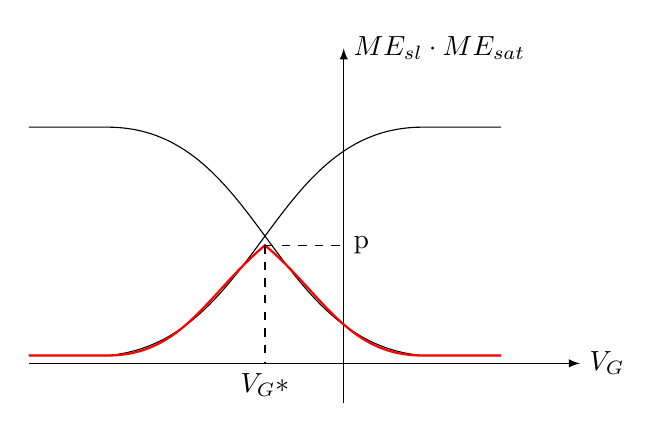
\begin{tikzpicture}
        %disegno asse x
        \draw[-latex](-4,0)--(3,0)node[right]{$V_G$};
        %disegno asse y
        \draw[latex-](0,4)node[right]{$ME_{sl} \cdot ME_{sat}$}--(0,-0.5);
        %disegno ME_sl
        \draw (-4,3)--++(1,0) to [out=0, in=175](1,0.1)--++(1,0);
        %disegno ME_sat
        \draw (-4,0.1)--++(1,0) to [out=5, in=180](1,3)--++(1,0);
        %disegno la loro moltiplicazione
        \draw [thick,red](-4,0.1)--++(1,0) to [out=0, in=220](-1,1.5) to [out=-40, in=180](1,0.1)--++(1,0) ;

        \draw[dashed](-1,1.5)--(0,1.5)node[right]{p};
        \draw[dashed](-1,1.5)--(-1,0)node[below]{$V_G*$};
    \end{tikzpicture}
    \caption{Caption}%
    \label{fig:enter-label}
\end{figure}
si trova il cosiddetto punto di massima efficienza. aumentare oltre la tensione di gate $V_G*$, peggiora le prestazioni. $V_G*$ è il punto di bias che pone un compromesso tra i due effetti /fenomeni di degradazione.

